\section{Implementation of the Scratch Detector}
In this chapter the development and results of a YOLOv5 solution for detection of scratches found on printed layers of a 3D binder jet printer will be presented. The following subsections will extend and go in-depth on the list of challenges presented in the introduction and present solutions and ideas to handle them.

\subsection{Labeling the Dataset}

\textbf{The first challenge:}
As mentioned in \ref{intro:challenges}, some scratches are weaker and should not be marked as actual scratches to not make the model too sensitive. A sensitive model would lead to many false positive detections like a thicker edge or an oxidation spot. The main goal would be to find a metric that can evaluate the prominence of the scratches. With such a metric, each annotated scratch will have a prominence value and therefore a minimum threshold could be used to eliminate the weaker scratches. \\

\textbf{The approach:}
A proper metric should measure how dark a scratch line is with respect to it's neighboring background. Also, the metric should not take in consideration the length or width of the scratch.
The metric developed for this project works as follows:
Crop the bounding box from the image. Because the image is a grayscale, the cropped image will have only 1 channel i.e. it can be interpreted as a 2D array. The rows of the array are normalized and the mean row is then calculated. For clarification: the mean row is obtained by summing all rows into 1 row and dividing each element of that row by the total number of rows. The center values of the mean row are usually lower than the values from the start or end of the mean row, because the bounding box has the scratch with darker pixels positioned in the center. The plot of the mean row would look like the hyperbole of $f(x)=x^2$. The mean row is then multiplied by -1 and the plot would look more similar to $f(x)=-x^2$, so it can be interpreted as single pulse of a signal. The prominence of this signal pulse can be calculated by using special signal processing functions like the ones provided by Scipy's module for signal processing \cite{scipy_signal}. \\
\begin{figure}[!h]
\centering
\captionsetup{justification=centering,margin=2cm}

\includegraphics[width=\columnwidth]{images/implementation/prominence_metric}
\caption{Sketch of the prominence metric computation.}
\label{impl:prominence_metric}
\end{figure}


Darker scratches will tend to have a higher prominence value than the faded ones. Now the only thing left to do is to choose a threshold and filter out the weak scratches. \\
During the filtering process, it was obeserved that some scratches had a surprisingly low prominence value. Usually, this was because the bounding box was not properly sized and the edges of a printed part were contained. Because the edges are dark, this would make the signal curve flatter and therefore the prominence value would be smaller. A resizing or centering of the bounding box solved this problem.

\begin{figure}[!h]
\centering
\captionsetup{justification=centering,margin=2cm}
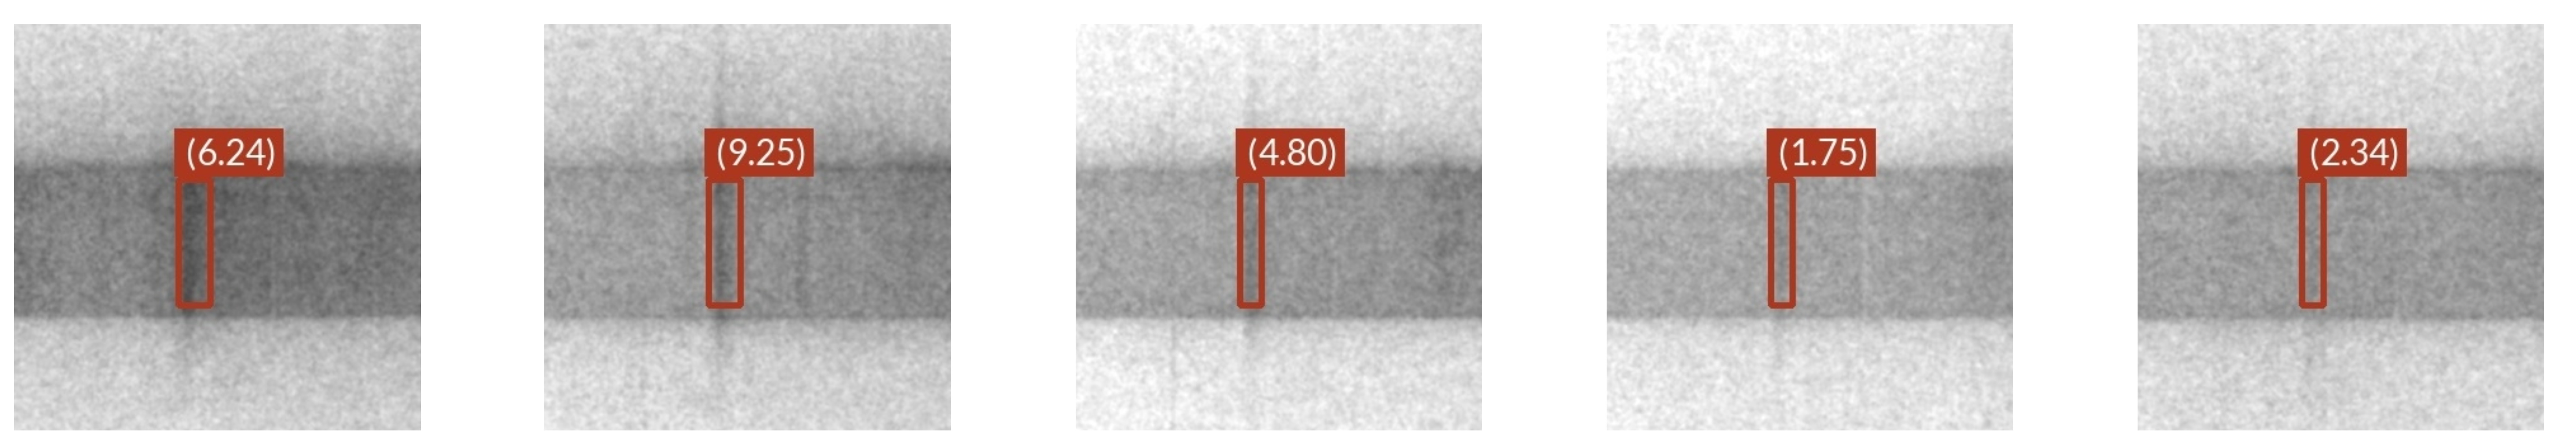
\includegraphics[width=\columnwidth]{images/implementation/marked_scratch_fades}
\caption{The prominence metric in action on the scratches from figure \ref{intro:original_scratch_fades}. Weaker scratch tend to have a lower score.}
\label{impl:marked_scratch_fades}
\end{figure}

\subsection{Bitmask Integration}
\label{subsection:bm}

\textbf{The challenge:}
As discussed in \ref{intro:challenges}, the images of the layers have two types of anomalies:
\begin{enumerate}
\item thick edges or closely positioned segments that look like scratches
\item artifacts from previous layer that look like scratches
\end{enumerate}

This situations might trick even humans and during labeling it was found out that each potential scratch had to be checked by looking the current bitmask and the previous bitmask. The current bitmask was used to check against the first type of anomalies and the previous one for the second type of anomalies. This lead to the intuition of integrating the bitmasks in the training process.
 However, most object detectors take as input exactly one image with the respective annotations. The challenge is to find a proper way to integrate the two bitmasks with each image and provide the model this extra context information.\\


\begin{figure}[ht]
  \centering

  \begin{subfigure}{0.75\textwidth}
    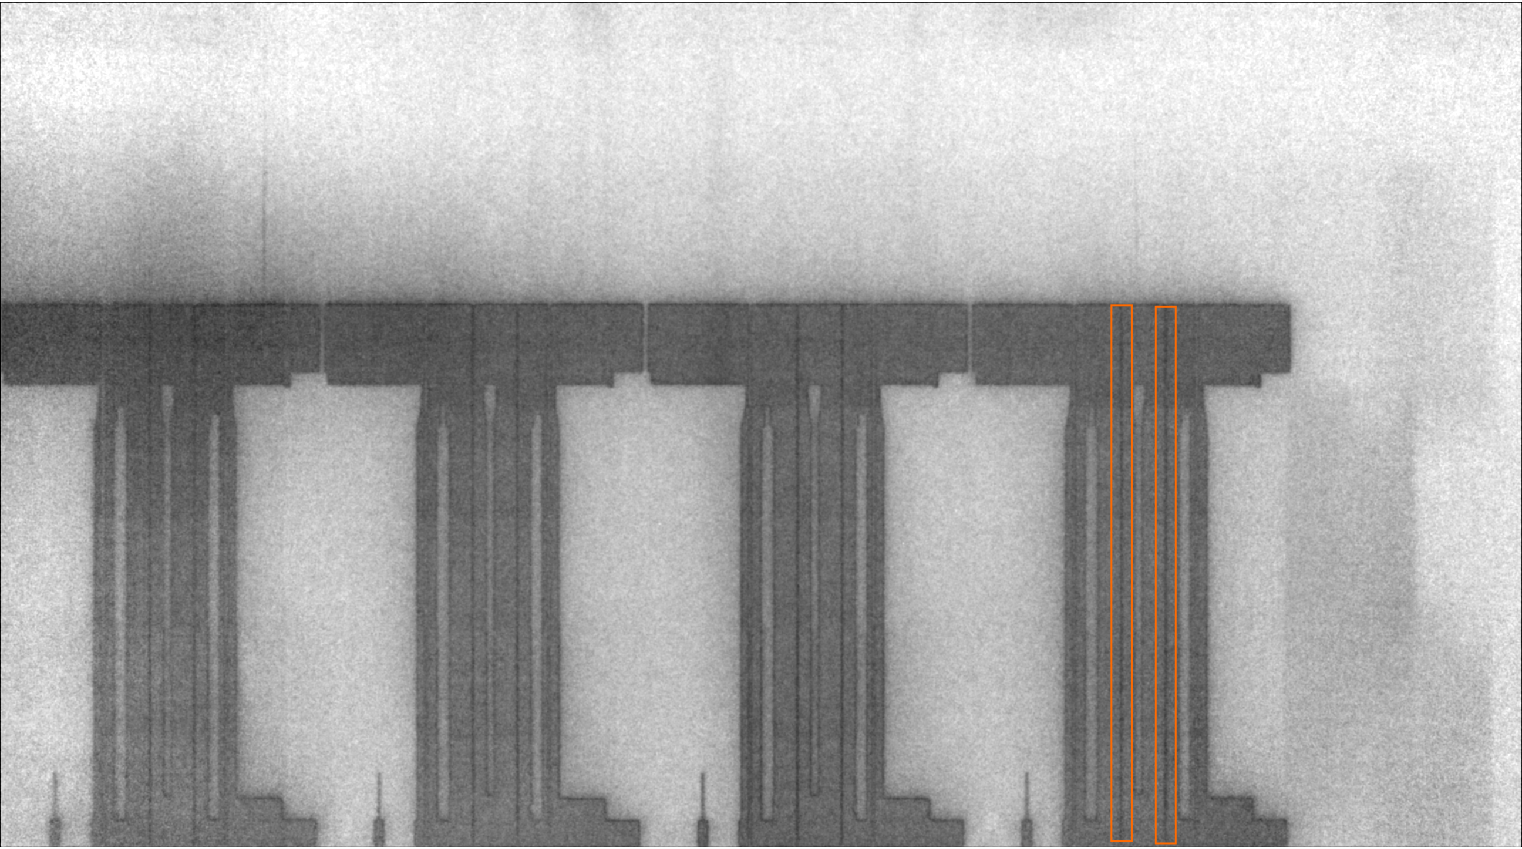
\includegraphics[width=\textwidth]{images/layer_01486_marked}
    \caption{Layer with thin splits marked in orange bounding boxes.}

  \end{subfigure}

  \begin{subfigure}{0.75\textwidth}
    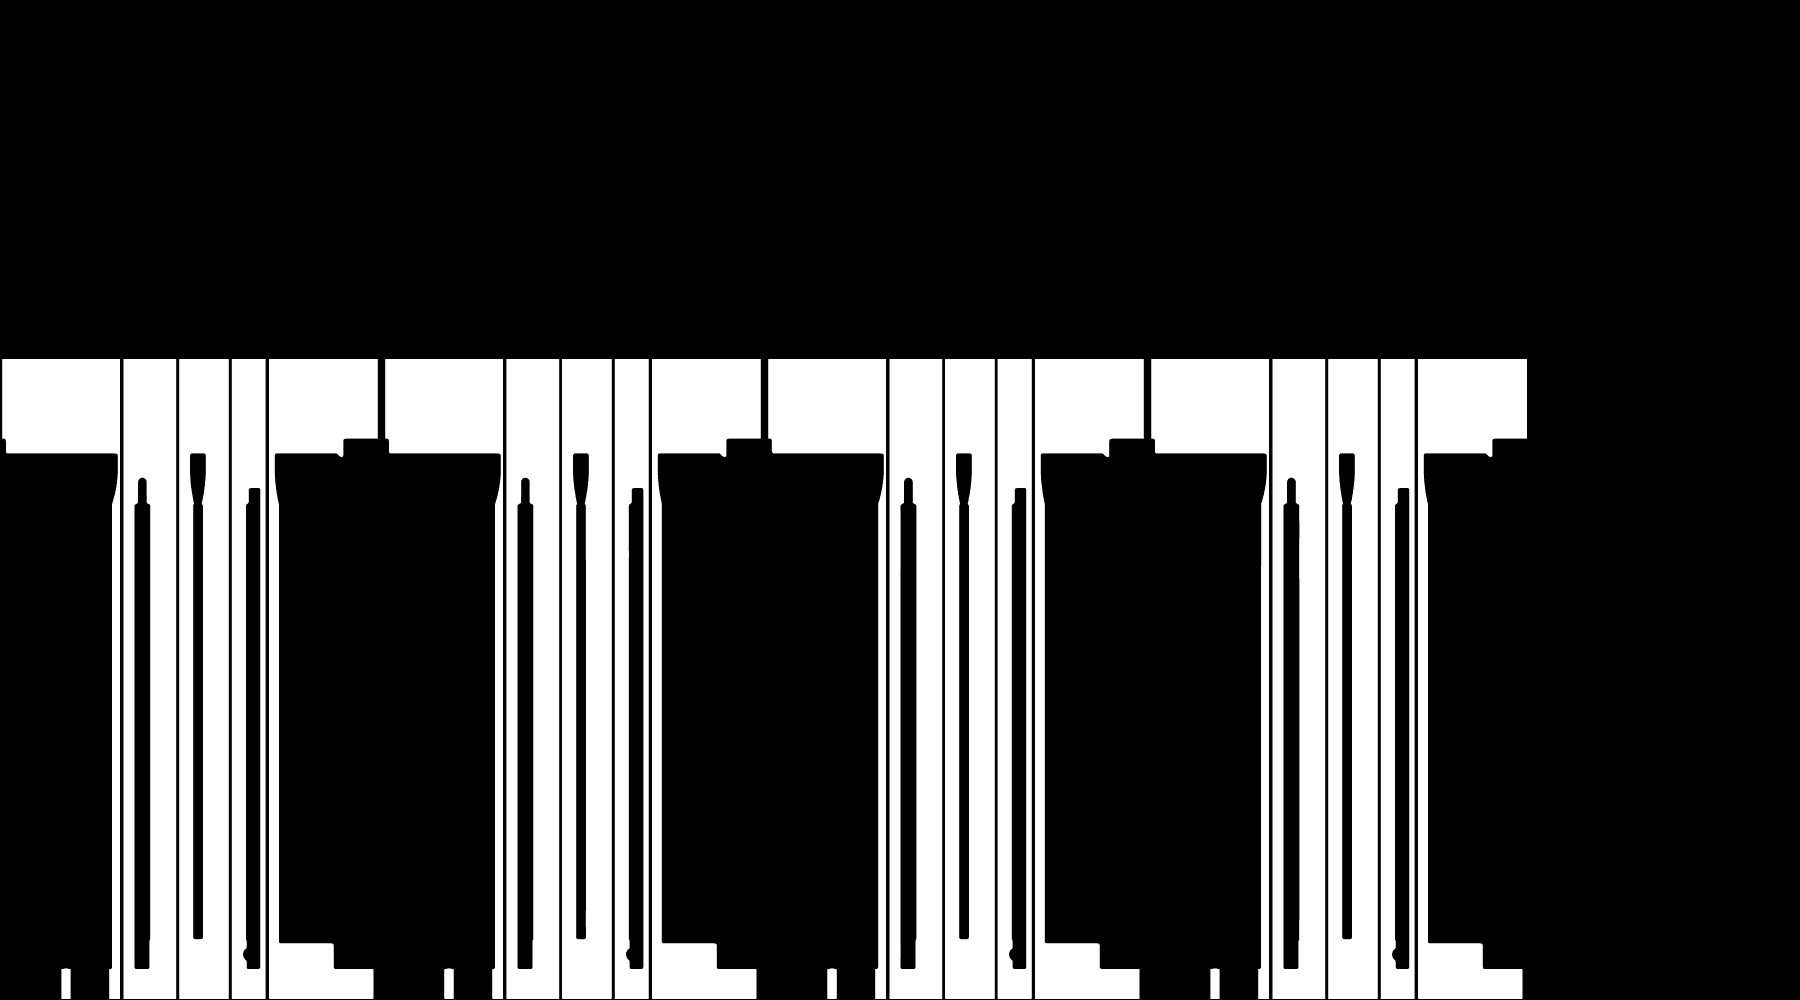
\includegraphics[width=\textwidth]{images/bitmask_01486}
    \caption{Corresponding bitmask.}
  \end{subfigure}

  \caption{The bitmask helps differentiating scratches from two closely positioned edges.}
  \label{fig:thin_splits}

\end{figure}
\textbf{The approach:}
YOLOv5 works with RGB images and if a grayscale input image is detected, it gets converted to RGB. This conversion provides no extra information and is more a preprocessing step.\\

A second conversion method is to represent the grayscale image with a single channel only and leave the other two channels empty. The two free channels can be then used to encode more context information related to image from the first channel. With the challenge statement in mind, filling up the other two channels with the current and previous bitmasks is clearly helpful e.g. the red channel contains the layer image, the green channel contains the current bitmask and the blue channel contains the previous bitmask. This is possible, because the bitmask images are also single-channel images. So instead of providing a grayscale image as an RGB image, three grayscale images are provided as an RGB image. If YOLOv5 gets a 3-channel image as input, then the pre-processing step made for grayscale images is skipped. \\

\begin{figure}[!h]
\centering
\begin{subfigure}{\textwidth}
  \centering
  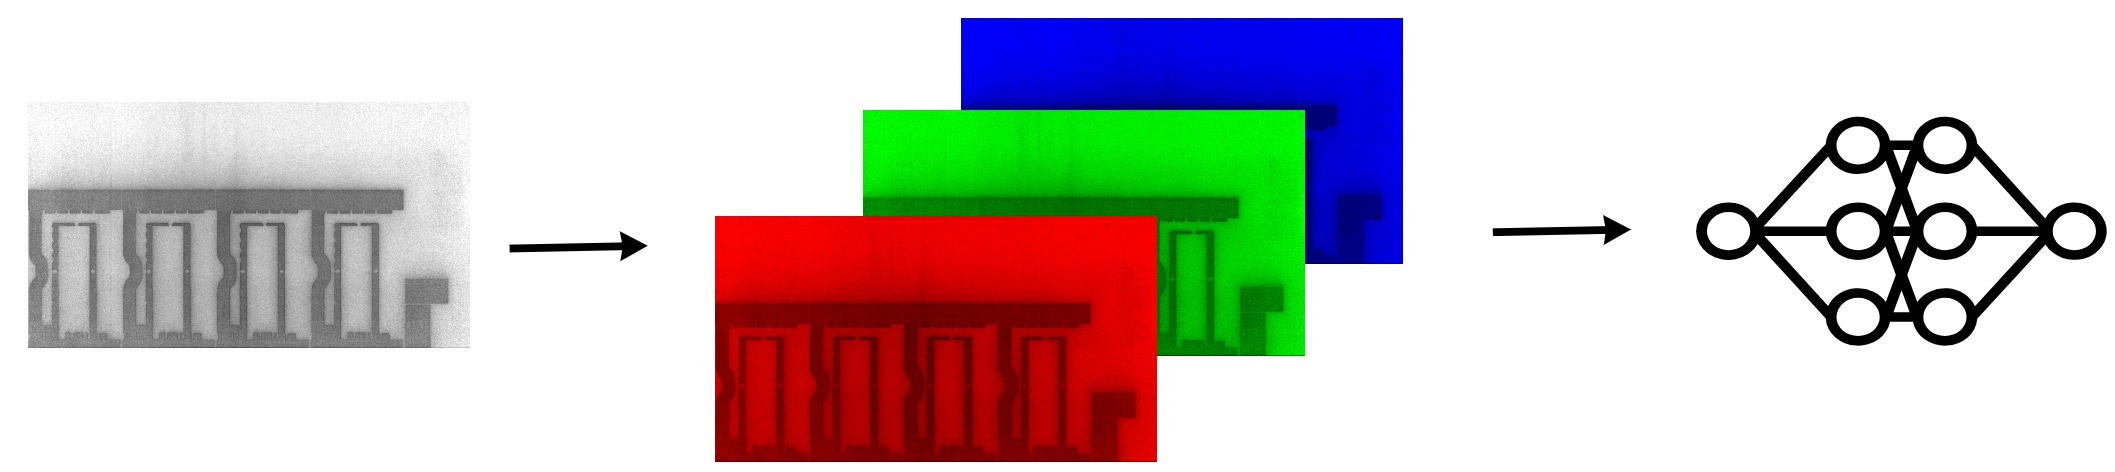
\includegraphics[width=\linewidth]{images/implementation/gray_to_rgb}
  \caption{Standard grayscale to RGB pre-processing.}
\end{subfigure}

\begin{subfigure}{\textwidth}
  \centering
  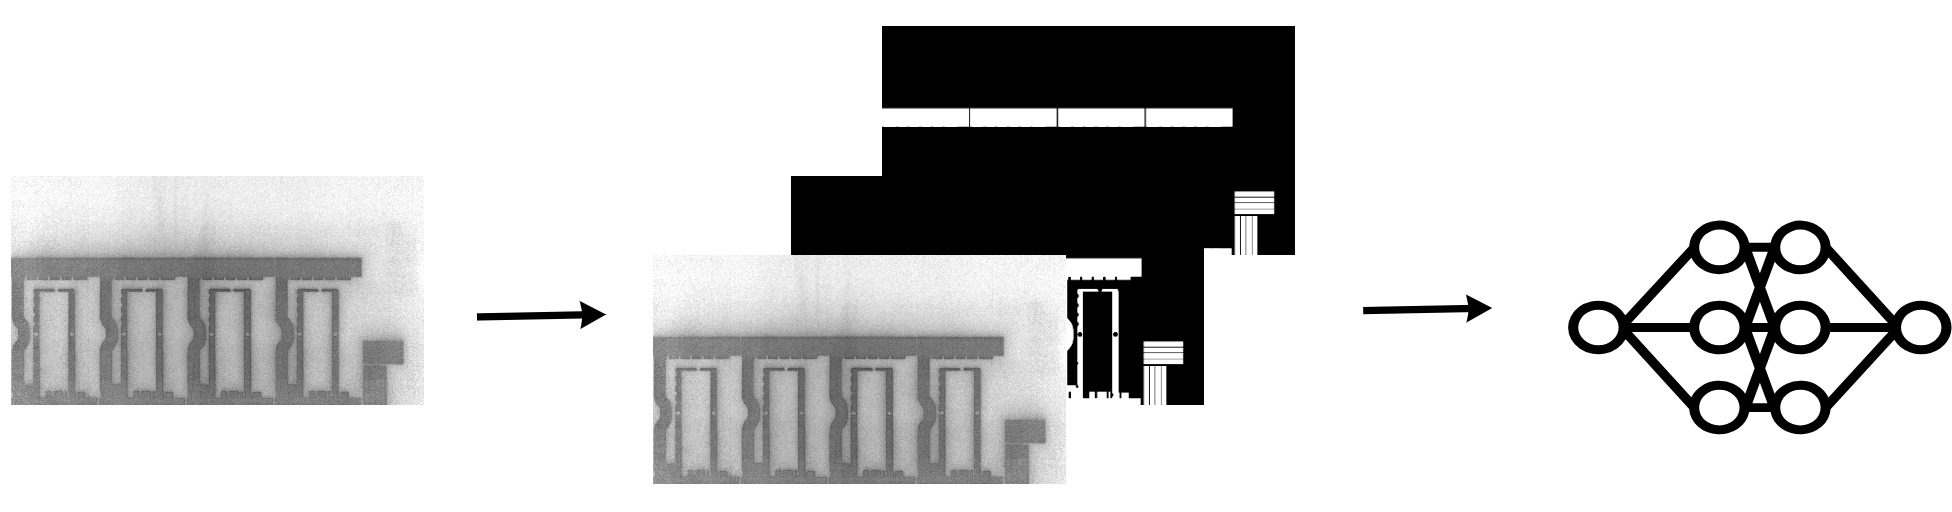
\includegraphics[width=\linewidth]{images/implementation/gray_to_bm}
  \caption{Custom pre-processing step for bitmask integration.}
\end{subfigure}
\caption{Visualization of the two different pre-processing steps.}
\label{}
\end{figure}


This new type of input image proved to make the model more robust against the above described anomalies, but with this new input some consideration and adaptations need to be made. \\
The layer images and the bitmask images have the same ratio, but different sizes of respectively 2592x1440 and 1800x1000. On one hand, the layer images can be downscaled to 1800x1000 and some image information is lost. On the other hand, the bitmask can be upscaled and the pixel-perfect edges get blurred. Another approach would be to meet somewhere in between e.g. downscale the layer images to 2196x1220 and upscale the bitmasks to 2196x1220. This trade off can be however avoided, if the the bitmasks are upscaled to the resolution of the layer images and a threshold on pixel values is used i.e. the pixels with a value below 0.5 are set to 0 and the rest are set to 1. The upscaled and thresholded bitmasks will retain this way all the pixel precise context information.  \\
Now the inference step will also need an extra pre-processing step to include the bitmasks and without them the inference is invalid. Also, the first layer is a special case, because it does not have a previous bitmask and the current layer is inserted twice. \\
This concept of filling the channels with context information was tested under many variations, but the one presented above delivered the best result. Most variations kept the original input image as the first channel and used different ways to fill up the other two channels. Some example of variations are:
\begin{itemize}
\item layer image and twice the current bitmask
\item layer image,the current bitmask and a logical OR of the current and previous bitmasks
\item layer image, the current Sobel-filtered bitmask and the previous bitmask
\end{itemize}
The first example does not include any information about the previous bitmask, so the second type of anomalies, the artifacts from previous layers, are detected as edges. The second example was problematic in some cases, because a logical OR of two bitmasks might treat a gap between two segments from the previous layer as a printed region. This leads to detecting a thin gap as a scratch. In the third example the initial intuition was that a Sobel-filter will directly show where the edges are, but the problem is that information about the current printed regions is lost. The list of variations is long, but those were some examples to get an intuition how context information is lost or malformed.

\subsection{Windowing}
\label{subsection:windowing}

\textbf{The challenges:} In the current release of YOLOv5 rectangular images are not that well supported. Data shuffling during training is available only for square input images, which is needed for a more robust training. Internally, rectangular images are actually padded to a square shape. This means that the images can be simply padded before using them as input to YOLOv5, but is the color or method of padding relevant? If so, how does this affect the training? \\
Another problem during development are questionable scratches like the ones that are positioned exactly on the edge and weird regions like oxidation spots. The easy way would be to simply ignore those images, but what if the image contains only one questionable scratch and three prominent scratches? The luxury of throwing away images is not very affordable with this small dataset. Remember that the dataset on hand is minuscule in comparison with open datasets. \\


The current images have a resolution way bigger than the average open datasets, so smaller batch sizes and/or longer training times are to be expected. Is there a way to use as training input only relevant regions of the images without losing any performance?\\

\textbf{The concept solution:} All the above problems can be solved by dividing the input image into smaller windows and training the model on those windows, called "windowing" for short.  However, there are many variables and considerations to be made:
\begin{itemize}
\item What is the optimal window size?
\item Is an overlap between the windows needed?
\item Are there any problems, if a scratch is not completely contained in a window?
\item What are the windowing strategies?
\item How to identify relevant windows?
\item How is the inference impacted?
\end{itemize}
The multiple sub-challenges together with those additional considerations make the topic of windowing more complex, but during this section an in-depth analysis of the windowing process will be made.

\subsubsection{Window Shape and Size}
As stated in the challenges, YOLOv5 is designed to work with square images. Using rectangular images disables data shuffling during and training and adds more potential side-effects with the padding of rectangular images to square images. The padding can have a color like the mean image color, or it can be a reflection of the last pixels. All those problem simply disappear, if the input image is subdivided into equally sized square windows. If needed, the neighboring windows might have an overlap to be able to use any desired window square size. \\
There are two types of images with respect to the count of annotations: normal images that have at least one annotation and background images that have no annotations. Because of the windowing, the number of background images can be quite large, but for the moment it is safe to not use them for training, because the official YOLOv5 documentations recommends a range of 0-20\% of the training dataset to be background images. \\
The next step is to take the right square size. Smaller windows will decrease the training time, and the questionable scratches and weird regions can be easily filtered out from training. The downside is that some scratches might get split into multiple windows and in some cases the splits are very unlucky e.g. one window might contains only 5\% of the original scratch. With bigger windows, the problems and benefits go in the opposite directions: the granular control of the scratch and region filter is lost, the training times increase, but the scratch splitting problem is less prevalent. The only constraint imposed by YOLOv5 is that windows width and length need to be a multiple of 32.\\
In set of tests the smallest window size was 320x320 and the size was increased then by 320 after each test. The final window size was 1280x1280. As it can be seen in table \ref{win_size_training}, the bigger window sizes provided the best mAP at the cost of higher training times. One surprising fact was that the 1280x1280 windows provided a stable and robust training, despite the fact that bigger windows are more likely to contain unwanted regions. This situations were actually rare, because the questionable scratches and weird regions were usually situated very far from the good scratches. This is a bit of a lucky situation. \\
 In table \ref{win_size_training} an overview of the datasets is displayed. An anomaly is the increase of window count for the 1280x1280 dataset, but this due the fact that the height of the original layer images is 1440 pixels and two 1280x1280 windows are required to cover the full height. Therefore, there is a huge overlap and for example a scratch in the middle will be captured by two windows instead of 1. This redundancy is not bad, because the same scratch is captured in two different coordinates. This is helpful for providing location variation of the labels.  \\
The avoidance of scratch splitting was somewhat helpful when training with bigger windows, but it seemed unlikely that this was the only contributing factor for better metrics, since scratch splitting occurred on less than 10\% of the total scratches. Also, the edge cases, in which the smaller split of scratch was below a threshold length, was filtered from the dataset. \\

\begin{table}
  \centering
    \begin{tabular}{ ||c|c|c||}
    \hline
    window size & seconds/epoch & total windows\\ [0.5ex]
    \hline\hline
    320x320 & 26 & 3328 \\
    640x640 & 35 & 1777 \\
    960x960 & 44 & 887 \\
    1280x1280 & 102 & 1214 \\
    \hline
    \end{tabular}
  \caption{Relevant stats for training on different windows size.}
  \label{win_size_training}
\end{table}

 A hypothesis is that larger windows provide more examples of scratch-free printed parts, which might contain some interesting cases like a darker edge or a gradient of gray. This in turn makes the model more robust. An initial naive approach was to put more background images in the 640x640 dataset, but the problem is that it even with the higher bound of 20\% background images it did not work. This is because many of the background images were irrelevant and did not contain printed parts. A second approach was to split each window of the 1280x1280 datasets into 4 640x640 windows. With this second approach, "double windowing", the results were similar to the experiment with 1280x1280 windows! The batch size on the double windowed dataset can be increased about 4 times, which leads to better batch normalization. \\

 \begin{figure}[!h]
 \centering
 \begin{subfigure}{0.33\textwidth}
   \centering
   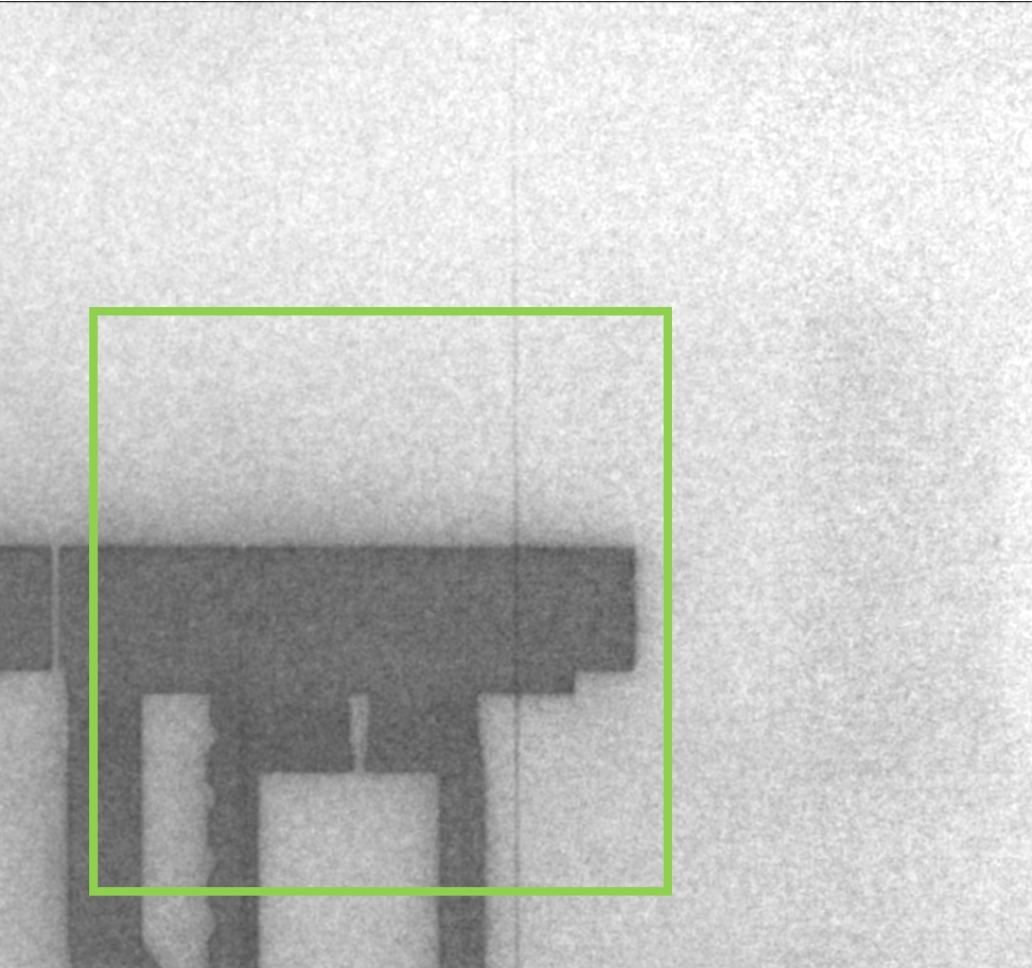
\includegraphics[width=\linewidth]{images/implementation/windowing/normal_window}
   \caption{Normal Windowing}
 \end{subfigure}%
 \begin{subfigure}{0.33\textwidth}
   \centering
   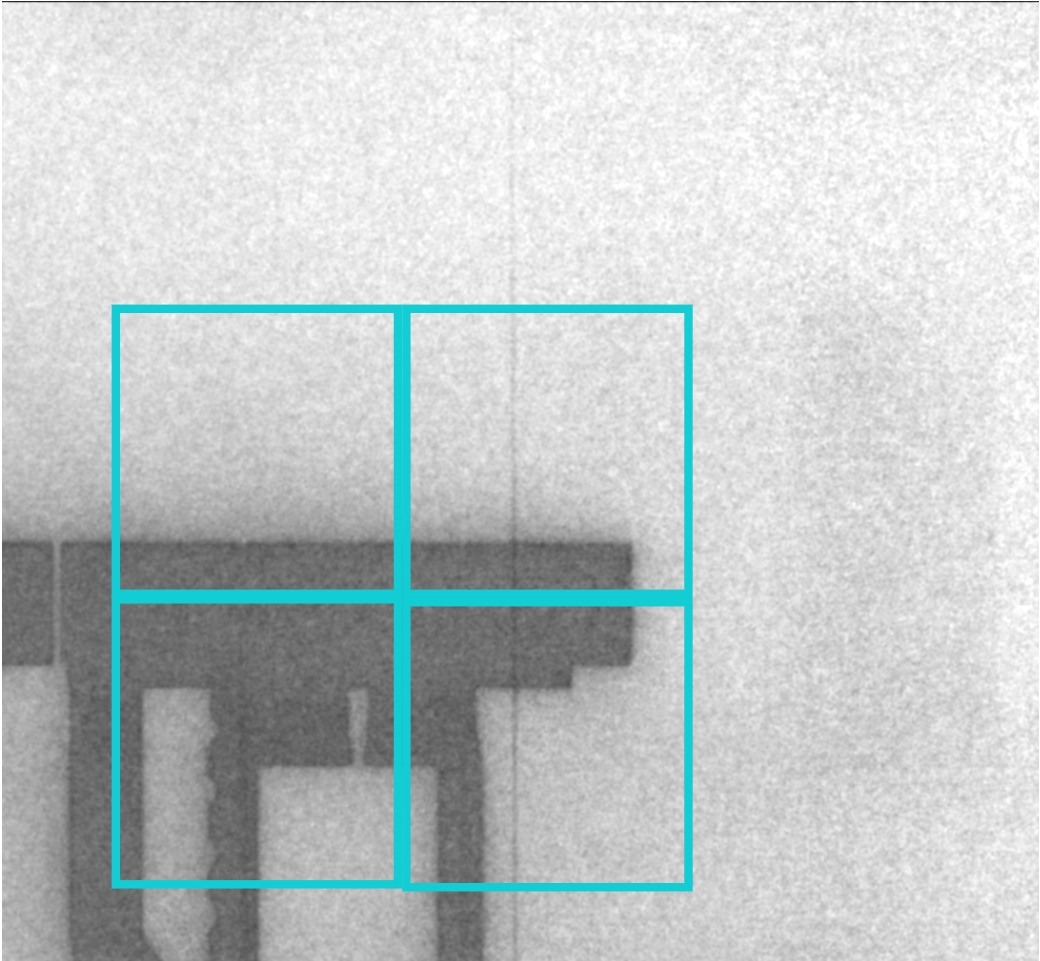
\includegraphics[width=\linewidth]{images/implementation/windowing/double_window}
   \caption{Double Windowing}
 \end{subfigure}%
 \begin{subfigure}{0.33\textwidth}
   \centering
   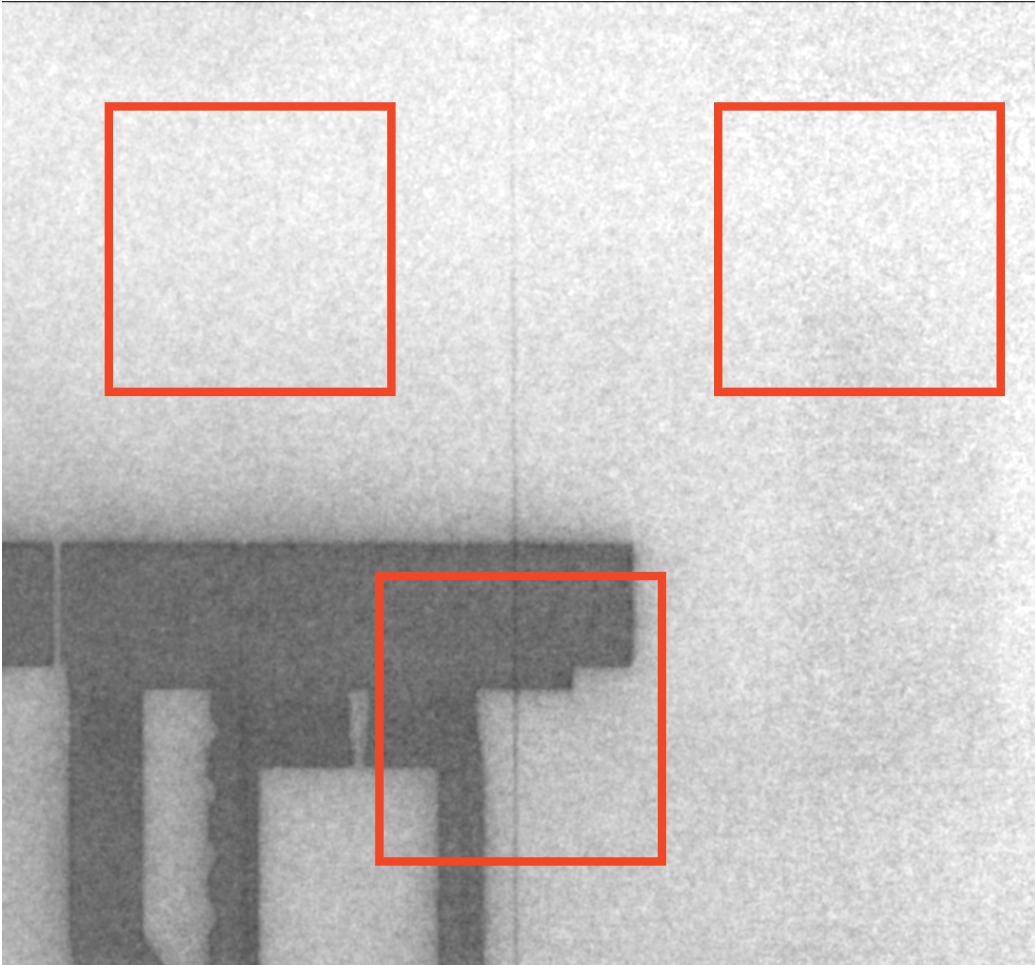
\includegraphics[width=\linewidth]{images/implementation/windowing/bckg_window}
   \caption{Random background}
 \end{subfigure}
 \caption{Visualization of normal vs. double vs. random background windowing methods. The blank background windows do not help the model learn about the printed structures.}
 \label{impl:normal_vs_double_bck_win}
 \end{figure}

Another interesting discovery is that it's helpful to mix the windows between the train and validation splits. This ensures a more similar distribution between the splits. The test dataset usually contains also the background windows that are needed for reconstruction and evaluation, so it's better to leave this split untouched. This observation alone stabilized the training experiments very much.  \\

\begin{figure}[!h]
\centering
\begin{subfigure}{0.33\textwidth}
  \centering
  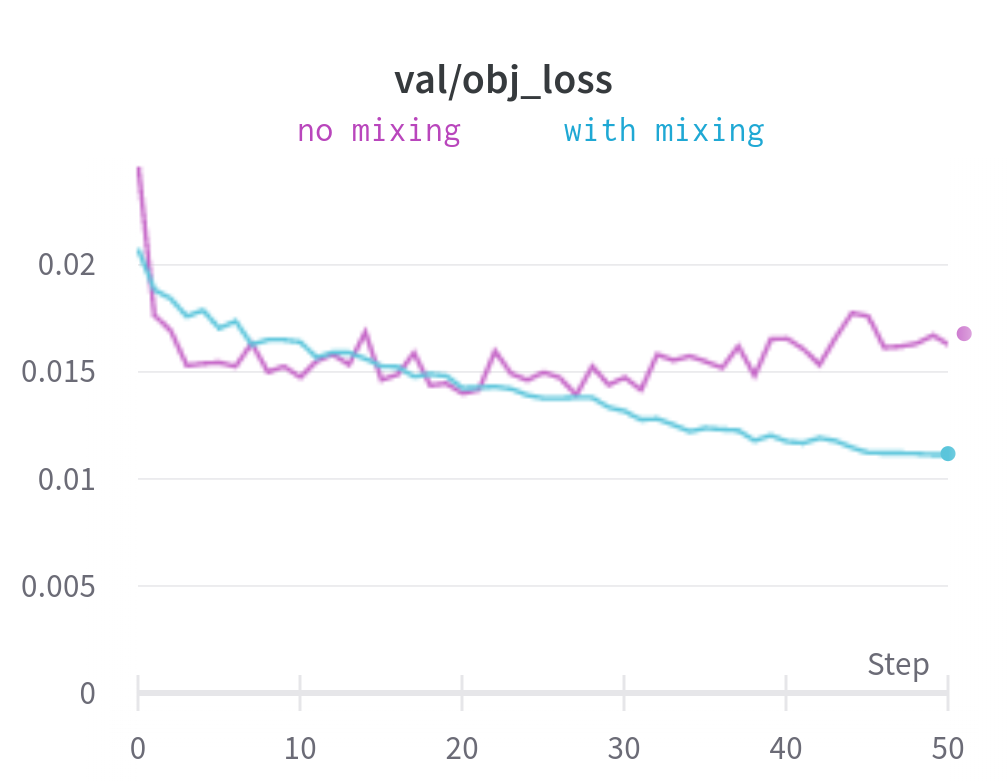
\includegraphics[width=\linewidth]{images/implementation/windowing/mixing/mixing_obj_loss}
  \caption{Objective Loss}
\end{subfigure}%
\begin{subfigure}{0.33\textwidth}
  \centering
  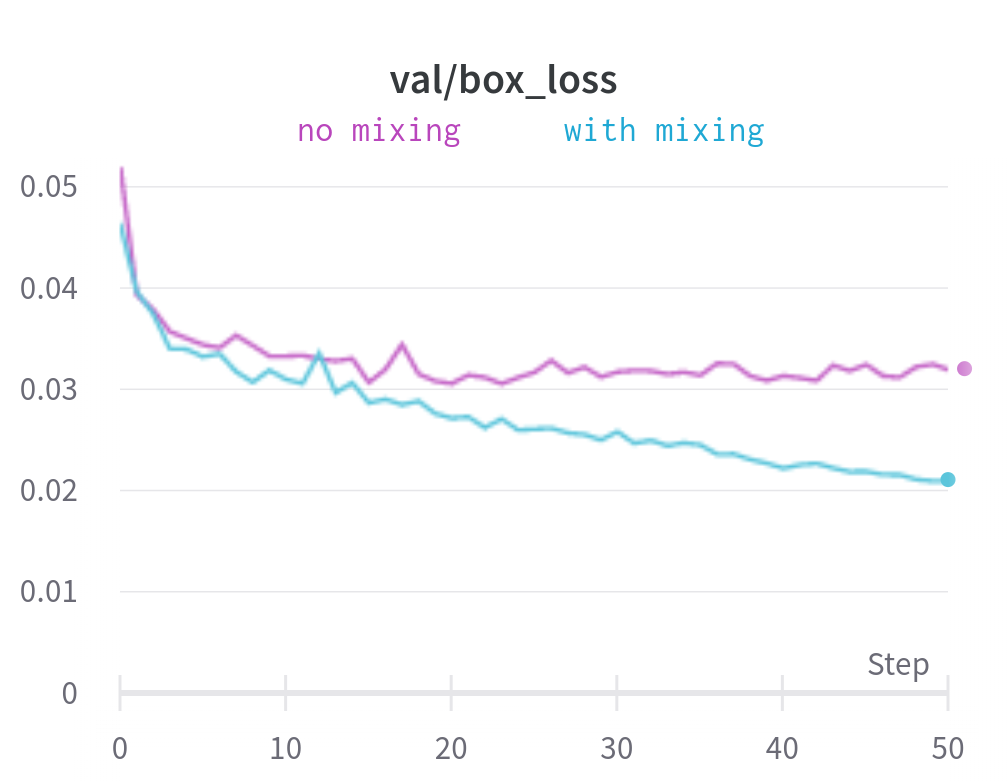
\includegraphics[width=\linewidth]{images/implementation/windowing/mixing/mixing_box_loss}
  \caption{Box Loss}
\end{subfigure}%
\begin{subfigure}{0.33\textwidth}
  \centering
  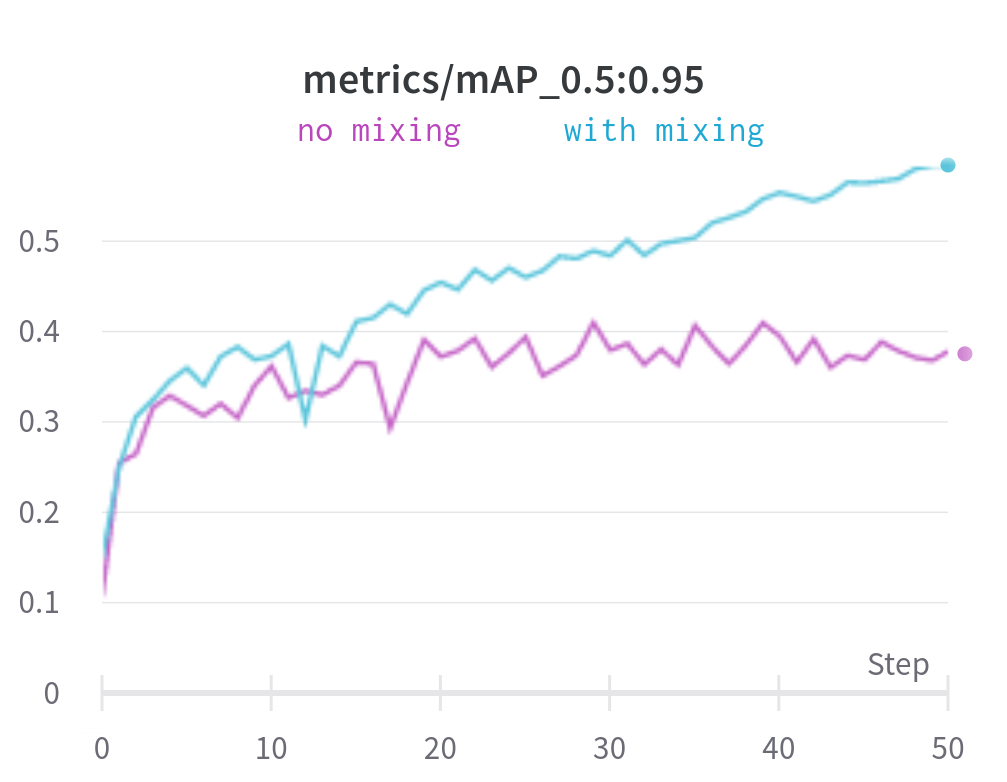
\includegraphics[width=\linewidth]{images/implementation/windowing/mixing/mixing_big_map}
  \caption{mAP@0.5:0.95 metric}
\end{subfigure}
\caption{With mixing the model does not overfit and metrics such as mAP are considerably better. In this figures step is meant as epoch. The respective MLOps platform uses this specific wording.}
\label{impl:mixing}
\end{figure}


\subsubsection{Windowing Strategies}
In the subsection from above a "grid windowing" strategy was assumed and as the name suggests, the corners of a grid are used to determine how to extract the windows. In a more advanced form, grid windowing also overlaps the neighboring windows. This helps avoiding the extreme cases of scratch splitting as seen in figure \ref{impl:scratch_splits}. One problem with grid windowing is that some layer are very similar to each other and also repeat the scratches at the exact same locations. This makes many windows to be repetitive.\\
A second window strategy, "random windowing", each scratch is initially contained in a window. The windows are then shifted randomly along the X and Y axis. This avoid the problem of repetitive windows described in grid windowing. \\
\begin{figure}[!h]
  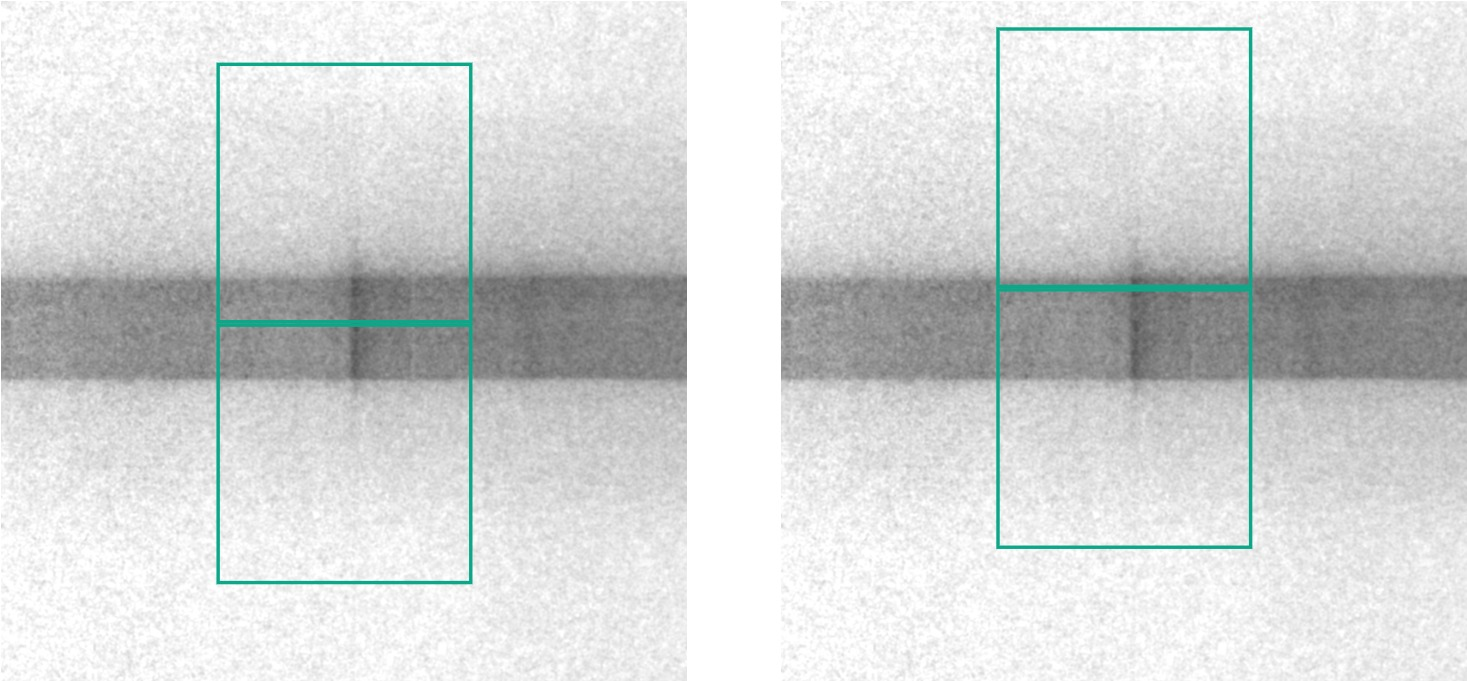
\includegraphics[width=\textwidth]{images/implementation/splits/scratch_splits}
  \centering
  \caption{Example of scratch splits. Sometimes a window might contain a micro-scratch and this cases can be handled in many ways e.g. by ignoring the label or dropping the window.}
  \label{impl:scratch_splits}
\end{figure}

\subsubsection{Adaptations for Detection}
If a model is trained on windows instead of the original images, some pre- and post-processing steps for detection need to be considered. \\
Before the detection, images need to be split in windows of similar shapes used in training. The strategy needs to be grid windowing, because all areas of the images need to be detected and this strategy makes reconstruction of the image easier. Also, an extra set of window between neighboring windows can be used to avoid scratch splitting. \\
After the detection, the windows with the respective detections need to be reconstructed to the original window. One naive way would be to draw detections on the windows and the reconstruct the windows into the original image. However, the trick is that with grid windowing every window has a predetermined position and the actual reconstruction of a new image can be avoided. In this implementation of grid windowing, the position of a window is specified by the upper left corner, width and height. This meta information can be easily encoded e.g. in the name of the file. Let's assume that a window of size 640x640 with the upper left corner at (500, 1000) contains a detection. This detection can now be translated by (500, 1000) and a valid detection for the original image is obtained. The translated detections can now be drawn directly in the original image.\\
Note that the detection is in YOLO format and the position of the initial detection is expressed in normalized coordinates with respect to the window size.Therefore, a conversion of the detection from the YOLO label format to COCO format \cite{coco_site} for the translation step is needed. After the translation, the detection can be converted back into the YOLO format.  Alternatively, the translation can be normalized with respect to the original image size.\\
The naive way is at least 2 times slower, but it still was able to deliver 1 FPS, which for this project is actually acceptable. A real-time detection is however possible with the second approach. The table \ref{impl:win_inference} shows the tradeoff between window size and inference time. \\

\begin{table}
\centering
\begin{tabular}{ ||c|c|c|c|c||}
\hline
window size & inference time & total windows & total layers & FPS\\ [0.5ex]
\hline\hline
320x320 & 106 & 10260 & 228 & 2.15 \\
640x640 & 60 & 3420 & 228 & 3.8 \\
960x960 & 44 & 1368  & 228 & 5.18 \\
1280x1280 & 100 & 1368 & 228 & 2.28 \\
\hline
\end{tabular}
\caption{Impact of windowing on inference.}
\label{impl:win_inference}
\end{table}

Another post-processing step after the translation of the detections is the merging of detections. Because scratches might get split, the respective detections should be some overlapping bounding boxes. Those bounding boxes need to be also merged. The problem is that sometimes the bounding boxes might not overlap at all and be even a few pixels apart and that is why a more generous overlap or an extra set of windows as shown in \ref{impl:extra_win} can be used used. This helps in connecting the disjointed detections. \\

\begin{figure}[!h]
\centering
\captionsetup{justification=centering,margin=2cm}
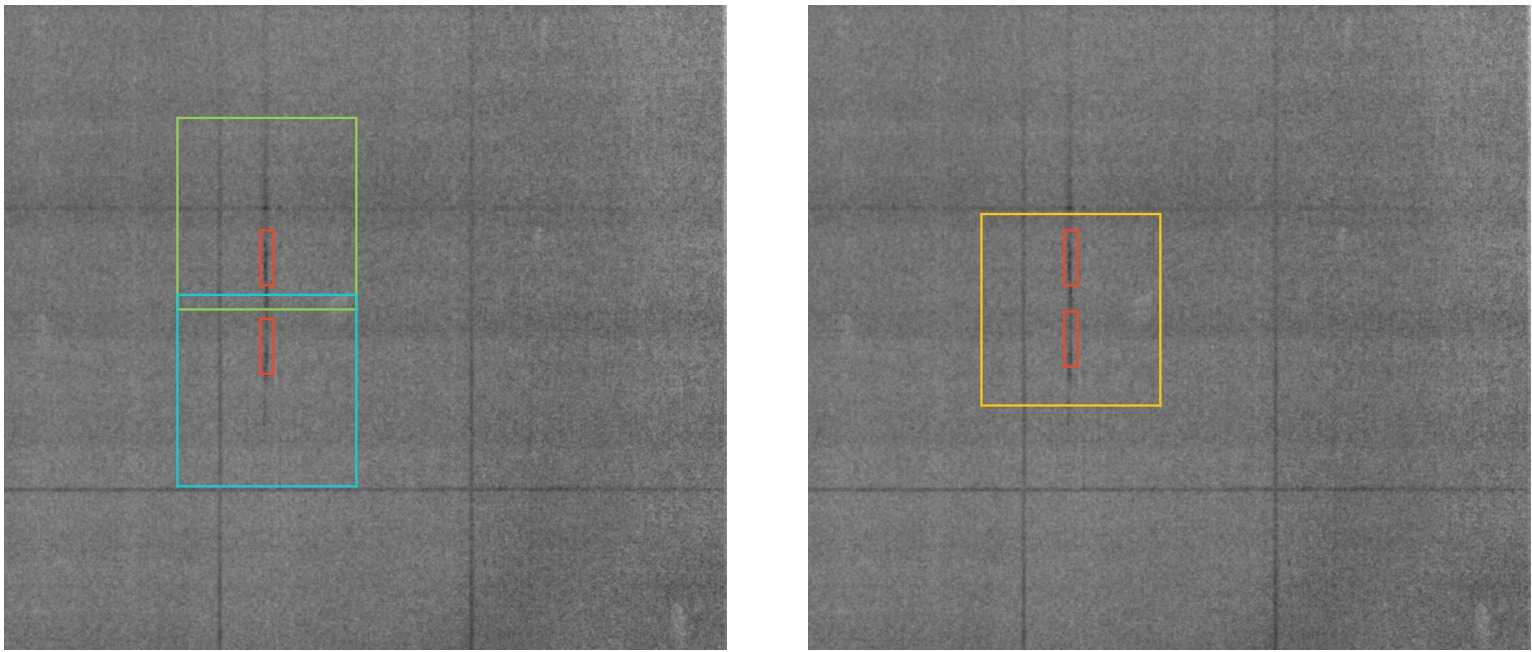
\includegraphics[width=\columnwidth]{images/implementation/extra_windows}
\caption{On the left: Example of a failed merge due to a small overlap between the windows On the right: Possible extra window to get overlapping detections. }
\label{impl:extra_win}
\end{figure}

\subsection{Augmentations}
The dataset at hand features a total of 2295 images of layers with the corresponding bitmask, but only a fraction of the images contain an actual scratch. This is far from the recommended minimum of 1500 images per class and 10000 instances per class. \\
It is important to make distinction between online and offline augmentations. With offline augmentations the images are augmented before the training and with online augmentation the images are augmented every epoch during the training. With a relatively small increase of training time, online augmentations provide a more robust training with the extra variance in the dataset, but sadly, not all augmentations methods can be implemented as online methods due to some technical constraints imposed by albumentations, the augmentation library used internally by YOLOv5 and YOLOv5 itself. The first constraint is that every augmentation method can have as input exactly one image with a list of bounding boxes. The second constraint is that the output is exactly one image with a list of bounding boxes. The third constraint is that the input image size needs to correspond with the output image size. \\
Basic augmentations methods like contrast and brightness manipulations are not affected by those constraint, but the random windowing is affected by this. Technically speaking, the random windowing is not an augmentation step, but it would be nice to be able to provide during each new epoch a new randomly shifted window for all scratches. This alone might stabilize the whole method and not face the fluctuations as seen in \ref{impl:win_strategy}.\\
Among the online augmentations, there is a special group that are able to circumvent some of the constraint. Those are some online augmentations that come out-of-the-box with YOLOv5 like CutMix and Mosaic. \\

\textbf{Mosaic:} The mosaic augmentation is an online augmentation that takes 4 images, which are randomly cropped and combines them into 1 image. This augmentation is built-in the YOLOv5 project and the constraint regarding the input for online augmentations is circumvented.
The input images are also downscaled at different rates, which helps increase the variance . A trade-off is that the new image actually contains smaller scratches, which raises the question if this has an positive or negative impact. This question is discussed in-depth in the paragraph about the stretch augmentations. \\
The parameters for this augmentation are only the probability of it being applies. The downscaling factors of the images, the number of the input images and the pick distribution are not parameterized. \\
Because of this unidimensional parametrization, the experiments were simply testing the effects of the mosaic augmentation at increments of 0.1 for the application probability. The results favored a application probability range between 0.5 and 0.8. This upper bound of 0.8 is a first indicator that the shrinking of the scratches might be problematic. Note that for higher application probabilities the results were actually ok e.g. the mAP@0.5 was only about 2\% smaller on average. The slightly more visible aspect was that for higher probabilities the bounding boxes were on average shorter, but still able to have an  IoU greater than 0.5. \\


\begin{figure}[!h]
\centering
\captionsetup{justification=centering,margin=2cm}
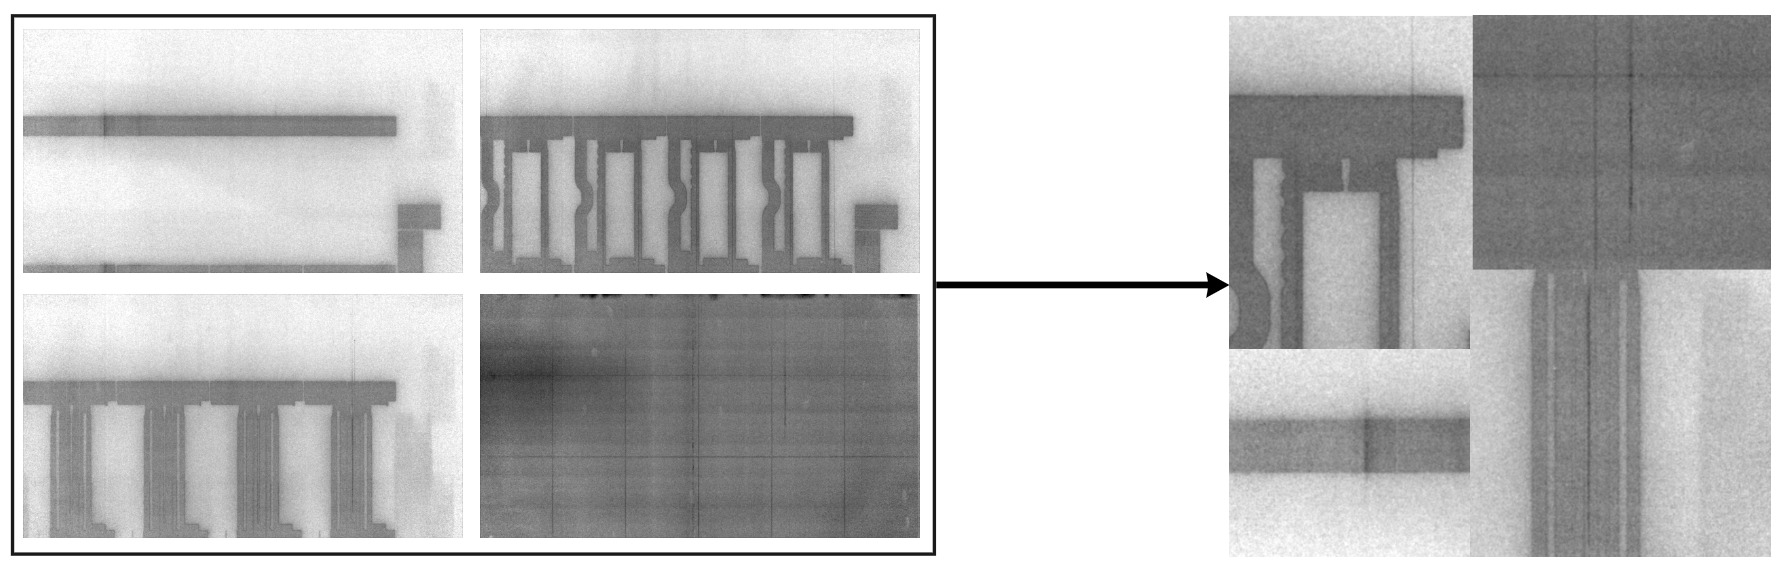
\includegraphics[width=0.8\columnwidth]{images/implementation/augmentations/mosaic_example}
\caption{Mosaic augmentation applied on the dataset on hand.}
\label{impl:mosaic}
\end{figure}

\textbf{Cut-Mix:}
The cut-mix is sometimes seen as mosaic augmentation with only 2 input images, but an important distinction needs to be made. The cut-mix crops a regions from an image and pastes it over the other input image at a random location. This was problematic, because sometimes the cropped region was partially or completely covering a scratch. The complet covering of a scratch is simply unwanted information loss and the partial covering was worse than the split scratches, because there is no way of filtering tiny splits like in the windowing process. \\
As before, the only parameter available is the application probability. Sadly, there is no way optimize/avoid the covering of scratches with the cropped image. For this reason this augmentation method was not used. \\

\begin{figure}[!h]
  \centering
  \captionsetup{justification=centering,margin=2cm}
  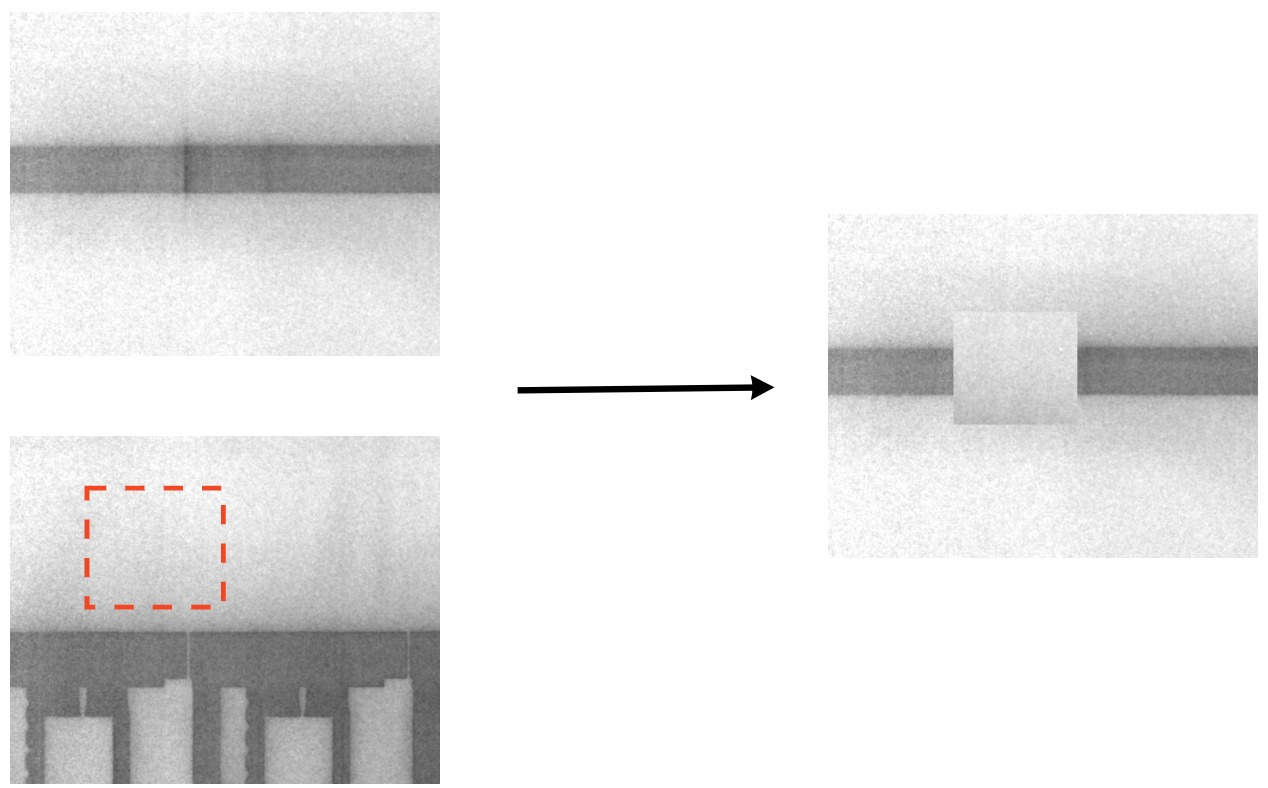
\includegraphics[width=0.75\columnwidth]{images/implementation/augmentations/cut_mix_example}
  \caption{CutMix augmentation that covers a valid scratch with a white background.}
  \label{impl:cut_mix}
\end{figure}


\textbf{Translate and Scale: }
Those two online affine augmentations are ok, if used carefully. Like before, they have only one parameter, but this time the parameter specifies the translation or scaling range e.g. 0.5 specifies a range of -0.5 to 0.5. For small ranges of up to +/- 0.2 for the translation and up to +/- 0.3 for the scaling the model trains with a nicely varied data. For higher ranges each augmentation had it's own problems. The translation moves the location of the scratch around, but image data is traded for black pixels like in figure \ref{impl:translation}. This reduces the amount of relevant background information that provide counter-examples for scratches e.g. thick edges. The scaling affects the average width of the scratch, which in the datasets barely varies by a few pixels. \\
Ideally would be to shift the window on the layer, so that the black regions are replaced with real data. The constraints of online augmentations make this impossible. \\

\begin{figure}[!h]
\centering
\begin{subfigure}{.5\textwidth}
  \centering
  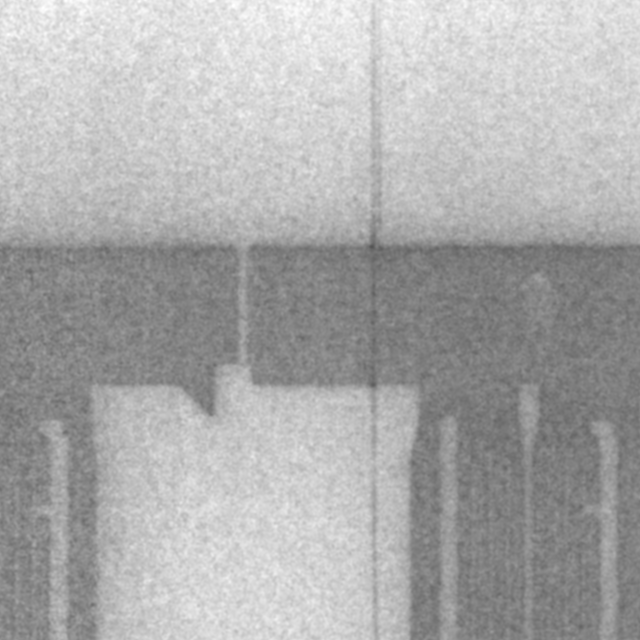
\includegraphics[width=.4\linewidth]{images/implementation/augmentations/window_no_translation}
  \caption{Normal window}
\end{subfigure}%
\begin{subfigure}{.5\textwidth}
  \centering
  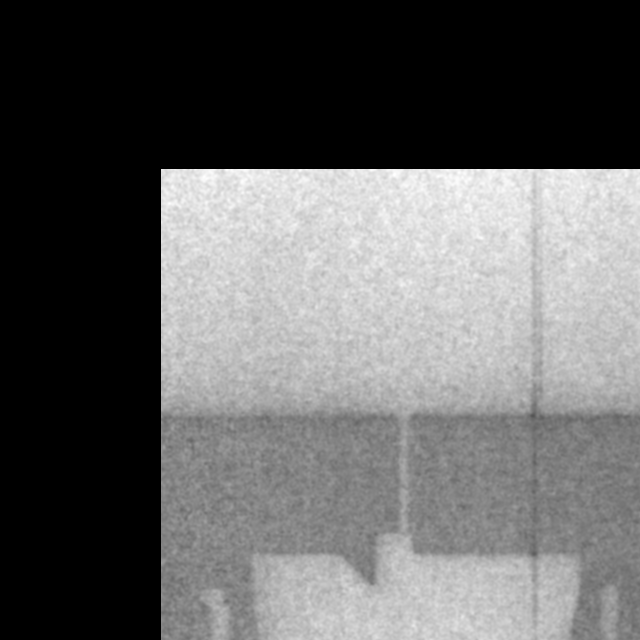
\includegraphics[width=.4\linewidth]{images/implementation/augmentations/window_translation}
  \caption{Translated Window}
\end{subfigure}
\caption{The translated window loses context information.}
\label{impl:translation}
\end{figure}



\textbf{Stretch and Squeeze:}
YOLO detectors usually have some hyperparameters the bounding boxes called anchors. The anchors are used as prior by the model for the location and shape of the bounding boxes. Ideally, before every training experiment the anchors need to be optimized with respect to the dataset. For newer YOLO versions this done automatically. With the help of windowing and translations the datasets contains a good variance for the positions of the bounding box and also the width barely varies. However, the length varies from 30 pixels to even above 600 pixels. Also, augmentations methods like mosaic tend to shrink the scratches and windowing introduces split scratches. This makes the training biased towards shorter scratches and the performance on longer scratches might be suboptimal. \\

\begin{figure}[!h]
\centering
\begin{subfigure}{.5\textwidth}
  \centering
  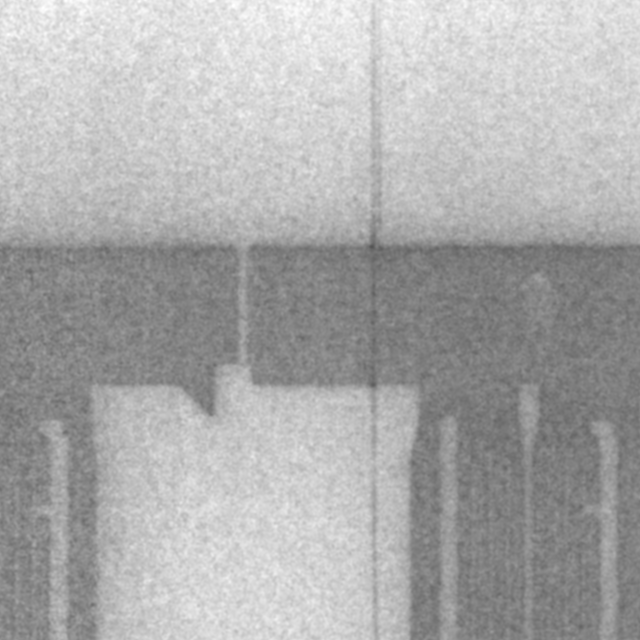
\includegraphics[width=.4\linewidth]{images/implementation/augmentations/window_no_translation}
  \caption{Normal window}
\end{subfigure}%
\begin{subfigure}{.5\textwidth}
  \centering
  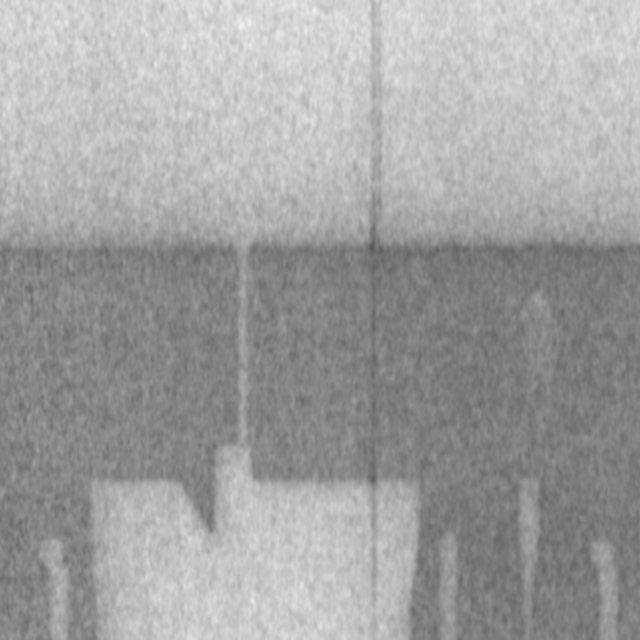
\includegraphics[width=.4\linewidth]{images/implementation/augmentations/window_stretch}
  \caption{Translated Window}
\end{subfigure}
\caption{The translated window loses context information.}
\label{sfdfsfsdfhf3}
\end{figure}

In order to test the hypothesis, if shorter scratches make the detection of longer scratches worse and vice-versa, an artificial dataset was used. Images were generated by drawing thin and long rectangles on a white background. For testing the hypothesis three artificial datasets, \textit{short scratches}, \textit{medium scratches}, and \textit{long scratches}, were generated. Then, the model was trained on those datasets, generating the corresponding weights \textit{short weights}, \textit{medium weights}, and \textit{long weights}. Each of the weights was then used for detections on each test split of the three artificial datasets. The results are seen in table TODO and it can be seen that YOLOv5 is more robust on detecting scratches from \textit{short scratches} dataset with the weights \textit{long weights}, than vice-versa, detecting on \textit{long scratches} with \textit{short weights}. Because the artificial dataset contains trivial examples, almost all the scratches were detected and the errors were mostly localization errors i.e. IoU below the 0.5 threshold. The IoU threshold can be lowered to 0.35, since a general localization is for this project good enough, but the problem of localization becomes a bit more serious, if the datasets images are split into windows. This is because the localization errors occur because the detected bounding boxes are shorter than the ground truth bounding boxes and for windowing this means that in some cases the detected bounding boxes might not overlap for neighboring windows, which leads to two small double detections in the original image. Therefore, there is a need to provide somehow longer scratches. The initial thought might be to use the scaling augmentation methods, but the method cannot be set to only scale larger and also the width of the scratch might be altered. \\
An alternative approach is to stretch the scratches by deleting a few upper or lower rows from the image and then resizing the image back to the initial size. This keeps the width unaltered. This stretch augmentation method is then used on the \textit{short scratches} dataset and it can be seen that the results on detecting \textit{long scratches} is improved. \\
This augmentation method needs to be augmented as a custom online augmentation method in YOLOv5. The current implementation uses only one factor that specifies at what rate the length of the image is reduced before stretching it back to the initial shape. \\

\begin{figure}[!h]
\centering
\captionsetup{justification=centering,margin=2cm}
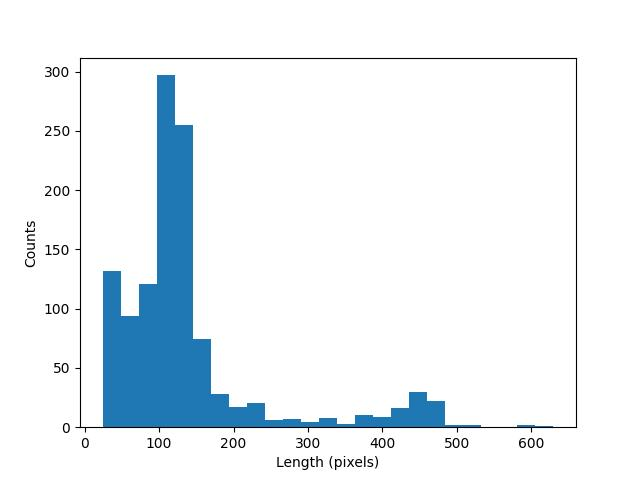
\includegraphics[width=0.6\columnwidth]{images/implementation/augmentations/scratch_length_histo}
\caption{Histogram of the length of scratches.}
\label{asdfsdf}
\end{figure}

The other way around is to use a squeeze augmentation method and this works by using windows that are randomly taller than the desired window height, then the windows are resized to the desired window height. This method is not possible to implement as an online augmentation method, because the taller windows cannot be squeezed due to the constraint of equal input and output size. Another approach might be to retrieve some corresponding upper or lower image rows of the respective window, but this is not possible, because the name/id of the window is not known. Therefore, this can be technically implemented only as an offline augmentation methods. \\

\begin{table}[!h]
\centering
\begin{tabular}{ ||c|c||}
\hline
scratch property & value (pixels)\\ [0.5ex]
\hline\hline
average length & 138 \\
median length & 117 \\
min length & 24 \\
max length & 630 \\
std. dev. of length & 110 \\
\hline
\end{tabular}
\label{impl:scratch_prop}
\caption{Statistic of the scratch lengths.}
\end{table}


\textbf{Contrast:} As stated in the introduction, scratches might be more or less prominent, but this effect can be in a way simulated with contrast changes. This method can be implemented as a custom online augmentation. The current implementation uses one parameter for the application probability and one parameter for the range of the contrast change. \\
In most experiments a contrast change of +/- 0.15 with any application probability helped the model be more robust and less false positive were detected. \\

\textbf{Flips:} Flipping means rotating the image around the vertical or horizontal axis. This simple, yet effective method prevents the model to look for a specific structure in the images. In the current use case, the scratches are not always perfectly centered in the bounding boxes. This might happen because most tools provide a usual feedback only after the drawing process of the bounding boxes begins. \\
YOLOv5 supports horizontal and vertical flips as online augmentations, but the implementation has some drawbacks. The double flip i.e. horizontal flip, followed by a vertical flips is not supported and if the image gets flipped, the original image will not be used for training. The original image is discarded, because of the constraint of a single output of online augmentations. \\

\begin{figure}[!h]
\centering
\begin{subfigure}{.5\textwidth}
  \centering
  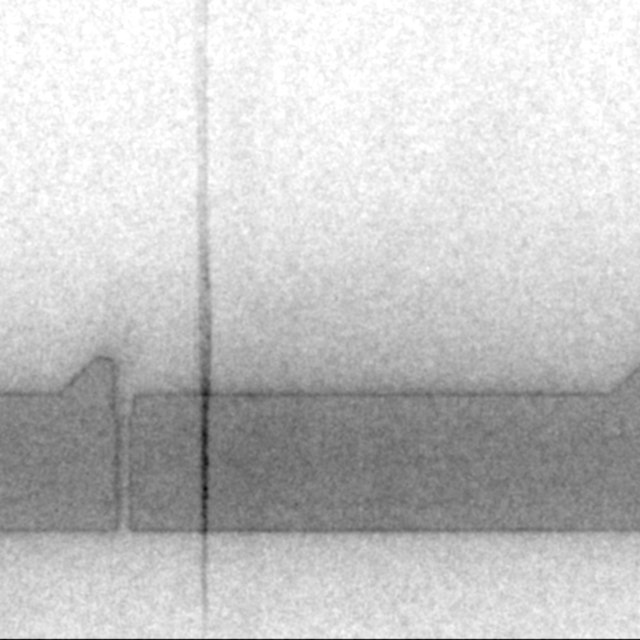
\includegraphics[width=.5\linewidth]{images/implementation/augmentations/flip_og}
  \caption{Normal Window}
\end{subfigure}%
\begin{subfigure}{.5\textwidth}
  \centering
  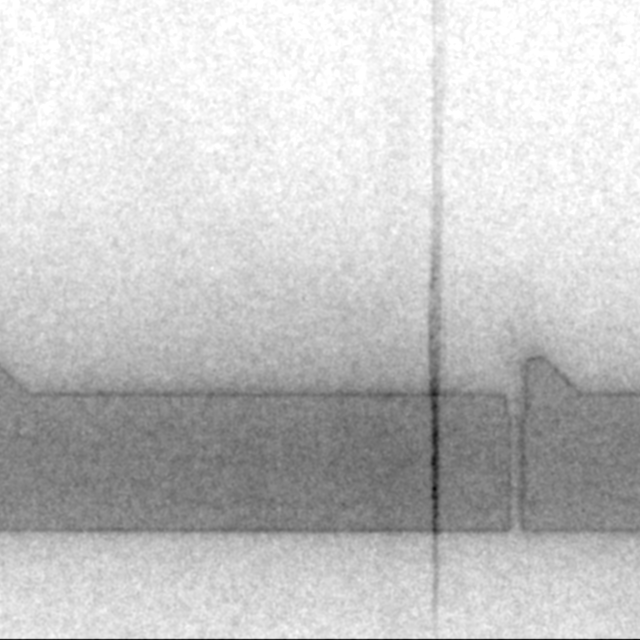
\includegraphics[width=.5\linewidth]{images/implementation/augmentations/flip_lr}
  \caption{Horizontal Flip}
\end{subfigure}
\begin{subfigure}{.5\textwidth}
  \centering
  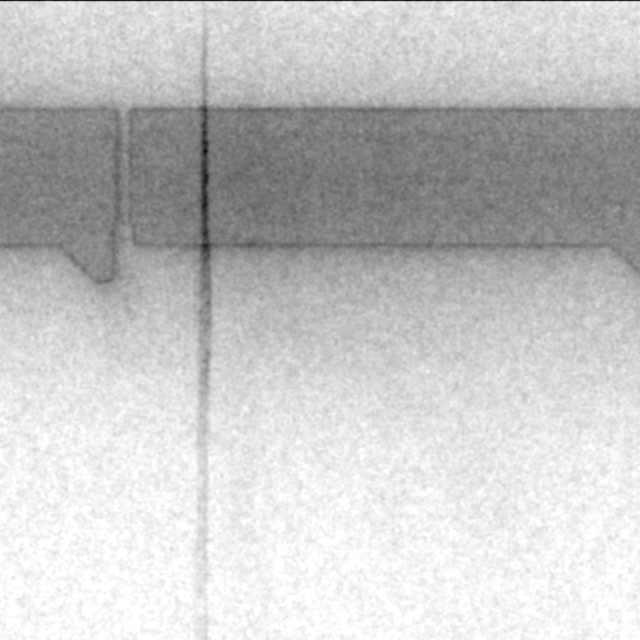
\includegraphics[width=.5\linewidth]{images/implementation/augmentations/flip_ud}
  \caption{Vertical Flip}
\end{subfigure}%
\begin{subfigure}{.5\textwidth}
  \centering
  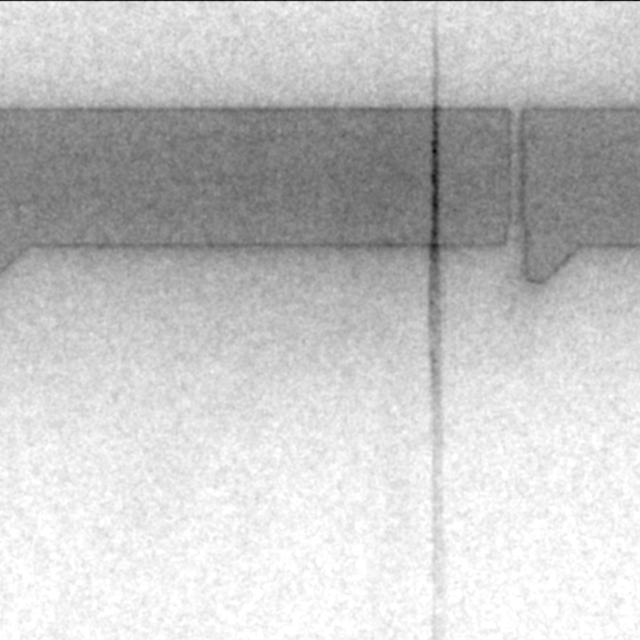
\includegraphics[width=.5\linewidth]{images/implementation/augmentations/flip_dbl}
  \caption{Double Flip}
\end{subfigure}
\caption{All possible flips of an image.}
\label{impl:flips}
\end{figure}


The aforementioned drawbacks lead to the development of an own offline augmentation method that supports the double flip. Because the single output constraint is avoided, the dataset may contain the original as well multiple flips of the image. In order to show the importance of using multiple flips, the results of 4 experiments are shown. In each experiment every window is augmented to a fixed number of flips and the results can be seen in table \ref{impl:flips_table} The worst performing experiment is clearly the one that uses a single flip version of the image and an improvement can be seen for each extra added flip. The biggest improvement can be seen at the mAP@0.5:0.95 and this means that the mode is able to better fit the bounding boxes. On average, each extra flips adds about 0.1 to this metric. \\

\begin{table}[!h]
\centering
\begin{tabular}{ ||c|c|c|c|c||}
\hline
flips per window & recall & precision & mAP@0.5 & mAP@0.5:0.95\\ [0.5ex]
\hline\hline
1 & 0.81 & 0.83 & 0.82 & 0.36 \\
2 & 0.84 & 0.85 & 0.85 & 0.45 \\
3 & 0.86 & 0.88 & 0.86 & 0.56 \\
4 & 0.91 & 0.93 & 0.02 & 0.66 \\
\hline
\end{tabular}
\caption{Training with different amount of flips.}
\label{impl:flips_table}
\end{table}

Flipping methods help the model become more robust in case the data does not contain diverse locations of scratches. \\


All the above augmentation methods are helpful for the given use case of scratch detections with the exception of the CutMix. Now the next paragraphs will discuss types of augmentations that proved to be affecting the general performance of the model.

\textbf{Occlusions:} The augmentation methods that end up occluding regions of the images should be avoided. As seen in the CutMix augmentation, this leads to loss or corruption of scratches. Popular augmentations methods that cause this type of occlusion are: Hide and Seek, CutOut, Random Erase and Grid Mask.

\textbf{HSV augmentation:} This augmentation is native supported by YOLOv5 and has three parameters that effect of the hue, saturation and value/lightness. By default the HSV augmentation is used for training and in theory benefits it should be helpful. The problem with this augmentation is that it cannot be used, if the bitmasks are integrated in the images channels as described in \ref{subsection:bm}. The HSV is essentially an alternative representation of the RGB color model, meaning that random modification of the hue, saturation and lightness will alter the bitmasks inserted in the color channels. For example, an altered bitmask might contain gray pixels on printed regions, instead of 1-valued white pixels and this might blur the precise context information provided by the bitmask. The upsides of integrating bitmask were tremendous and therefore the HSV augmentations will be deactivated.

\textbf{Shears and Rotations:} One main characteristic of the scratches is the verticality. Image shearing or rotations will generate images that are outside of the distribution and will force the model to learn about scratches horizontal and diagonal scratches that do not actually exist. Another problem is that the anchors of the bounding boxes will not be properly optimized, because a diagonally placed scratch will not a shorter and wider bounding box. This mean that the fitting of bounding boxes will get worse.

\textbf{Image Perspective:} This augmentation has negative effects on a similar note to the shears and rotations. In the given dataset all images are captured from a perpendicular perspective since the camera is positioned directly above the center of the powder bed. Changes in the image perspective will generate images outside of the distribution. \\
Perspective changes will also affect the verticality of the scratches, which affects the anchors of the bounding boxes and generates unreal data. \\

\textbf{Hidden Augmentations:}
In the current implementation of YOLOv5 there is a hidden pipeline of augmentations that are generally bad for the use case of scratch detections. The hidden detections are:
\begin{enumerate}
\item Blur and Median Blur: This affects the sharpness of the edges and the model does not learn to distinguish a thick edge from a scratch
\item Grayscaling: This converts the image to a single channel image and therefore the new compressed images fail to provide context information from the integrated bitmasks.
\item CLAHE (Contrast Limited Adaptive Histogram Equalization): This one tries to reduce the noise of an image and it ends up removing very faded scratches or making the oxidation marks very dark. This will make the model see less edge cases. \\
\end{enumerate}
The application probability is only 1\% for all, but they still might confuse the model with the altered bitmasks and less expressive images. Those are used as an example for creating a custom online augmentation with \textit{albumentations} and the best way to deactivate the augmentations it to delete the provided example. Technically, if the \textit{albumentations} library is not installed all the custom online augmentations are disabled, but this will disable also the self implemented augmentations like the contrast, which is definitely not a good idea.

% TODO images from \ref{roboflow_yolov4_augs}
% TODO What is the Bag of Freebies in YOLOv4?
% TODO talk about Bag of Specials

% TODO talk about anchors in YOLO in detection.tex

\subsection{Two Stage Training}
\label{subsection:two_stage_training}
The false positive were most of the time the bigger problem than the false negatives. With windowing the model has on average multiple chances to detect the same scratch due to the overlapping of the windows and therefore less scratches are missed. To push down the number of false positive, a two stage training approach can be used to feed the false positives to the model as a negative class. Note that this should not be confused with a two stage detection. \\
In two stage training two datasets are used. The first one contains no background images, but the second one extends the first dataset by containing all the background windows too. Remember that for YOLO a background rate of 0-20\% is recommended, so only the first dataset can be normally used for training. Now the model can be trained a first time on the first dataset. Then an inference is performed on the second dataset and the false positives can be all marked as a second class. Now a third dataset is created, which contains the newly obtained 2 class labels, but also with no background windows. This dataset in an enhancement of the first dataset by marking all the false positive with a new class and introducing background windows that might further contain false positives. Finally, a second training experiment is performed with the third dataset. \\
% TODO drawing of 2 stage training \\
This way the model learns in the second stage from the mistakes in made in the first stage and from relevant background windows. The similar concept of introducing meaningful background images can be seen also at \ref{subsection:windowing} with the \textit{double windowing} approach. The metrics on the second class are not very important, because this class is not really a class of objects, but rather a sinkhole for outliers and unexpected cases. One example of an unexpected case is the presence of a black border in the images. Those black borders can be eliminated in a pre-processing step, but then this pre-processing step needs to be also integrated in the inference. Also, this pre-processing steps might involve future manual adjustments, if in future datasets the border becomes thicker or thinner. With a two stage training approach all those cases can be learned by the model and manual tuning is avoided.\\
After the second stage the initial number of false positives drops by 80\% on average, but there is a slight problem with the metrics and validation losses. Because the second class is actually a sinkhole, the metrics and validation losses from this class do not have a relevant meaning. Because YOLOv5 outputs by default the metrics and losses aggregated and not for each class individually, it is difficult to track the second training experiment. \\
% TODO drawing of 2 stage training alternative or maybe combine with the one above\\
An alternative way for the 2 stage training is that the after creation of the third dataset, the labels for the second class can be deleted, but the respective windows are kept. This way the model gets to see the outliers and tricky cases without using a second class. This way the second training experiment can be then properly monitored. The downside of this approach is that the false positive rate drops by only 60\% on average, because there is no bounding box to specifically mark the problematic situations. \\
The two stage training is a process that can learn to be more robust and in the end it does affect the inference time. In YOLO specific terms, this technique is considered a \textit{Bag of Freebies}. \\



\subsection{Hyperparameters}
The default hyperparameters are set in accordance to the \textit{model size} and on normal datasets should get acceptable datasets. The dataset of scratches deviates from the usual datasets by the relative tiny size, usage of color channels for context information and size ratio of the bounding boxes. Therefore, the default hyperparameters do not deliver good results as seen on open datasets. \\

\textbf{Model Size and Type:}
YOLOv5 comes in 5 sizes: nano, small, medium, large, extra large. The nano models are targeted for edge and mobile devices, so for the current use case nano models are not suited.
During initial stages of development small and medium models were used to quickly explore initial hypotheses, but later on the models were upgraded to medium and large size. As expected, larger models generalized better, but with increasingly higher training and inference times. The extra large model was able to provide a few FPS, so there should be no worries about the increased inference time. \\
There also two types of models, the normal ones and the P6 models. The difference it that the normal models have three output layers called $P3, P4, P5$, while the P6 models have also a fourth layer called $P6$. The P6 models showed consistently a slightly higher mAP@0.5:0.95 of about 0.02, all this without adding significant increase in training time. Therefore, the P6 is the default network type in all experiments showed.

% TODO table with epoch times
% TODO show big mAP plots

\textbf{Weights:}
For a unique dataset that contains bounding boxes with a disproportionate shape ratio and context information encoded in the color channels, a training from default weights seems very promising, but this works only if the dataset is very large. The only solution is to use the pretrained weights, which provided better results than the default weights.  \\
% TODO show plots

\textbf{Hyperparameter evolution}

\textbf{Batch Size:}
The official documentation recommends that training should be performed on the biggest batch size possible in order to produce the best batch normalization statistics, but meanwhile on the official Github repository the developers suggest that YOLOv5 is batch agnostic. For the sake of finding the truth, multiple experiments with varying batch sizes have been made. The results were that for batch sizes up to 64 the map@0.5:0.95 metric was in favor of bigger batch sizes. Other metrics had no tangible differences. Bigger batches required more than 2 GPUs or compromising to a smaller window size.
The explanation is that higher batch sizes help with a better batch normalization. \\
% TODO show results \\

\textbf{Learning Rate and Gradient:}
The initial experiments showed high jumps after each epoch, so a switch from the standard stochastic gradient descent to AdamW has been made. The documentation recommends for AdamW to change the learning rate from 0.01 to 0.001, but a step size of 0.0001 showed a more stable evolution from epoch to epoch.
% TODO maybe show some results

\textbf{Loss Function:}
The loss functions has three components:
\begin{enumerate}
  \item class loss
  \item box loss
  \item objective loss
\end{enumerate}
%source https://github.com/ultralytics/yolov5/issues/5401

For the class loss the Binary Cross Entropy (BCE) loss is calculated for each class individually and then all individual BCE class losses are summed together. This sum can also be scaled by an optional coefficient. The available hyperparameters are the BCE positive weights coefficient $cls\_pw$ and the optional sum coefficient $cls$. The BCE positive weights coefficient acts  only on the true positive cases. In general if $cls\_pw>1$ the number for increases recall and decreases precision and if $cls\_pw<1$ then it works the other way around. \\
The class loss is only relevant if multiple classes are used, just like in the second stage of the two stage training approach. The $cls$ hyperparameter should be in this case low, because the second class is actually a sinkhole correcting mistakes from the first stage. The recall is usually not a problem, because the scratch may appear in multiple windows, so the model has multiple chances to detect the same scratch. With this observations in mind and some training experiments, it has been found that for the second training stage the class loss hypermeters should be as $cls\_pw \in [0.75, 1.0]$ and $cls \in [0.0, 0.2]$ \\
The objective loss is computed in a similar way by computing the BCE loss for each image and adds each image loss into a sum. The difference is that the objective loss is calculated on an images basis, while the class loss is calculated on a class basis. The hyperparameters available are $obj\_pw$ and $obj$, which are applied just like the $cls\_pw$ and $cls$ hyperparameters, respectively. In order to combat the high rate of false positive a $obj\_pw \in [0.5, 0.9]$ is optimal. To heavily punish the false positives and false negative a $obj \in [1.5, 2]$ is optimal. \\
The box loss is used to calculate how good the predicted bounding boxes are fitted to the ground truth bounding boxes. This loss is based on the Generalized Intersection over Union (GIoU). The box loss has only on hyperparameter available, $box$, which acts as scaling coefficient for the loss. The pixel perfect localization of the bounding boxes is not the main point of this project and usually a 70\% of the default value is a good value. \\
After the objective and class loss, the Focal Loss (FL) \cite{focal_loss_paper} function is applied. The goal of this function is to shift the focus from positive to negative examples and this can be tuned the $fl\_gamma$ hyperparameter. Usually, a $fl\_gamma \approx 0.5$ is good. \\
The general loss function with the respective hyperparameters can be sketched as:

\begin{equation}
  \begin{array}{l}
    L_{obj} = FL(obj * BCE(obj\_pw)) \\
    L_{cls} = FL(obj * BCE(cls\_pw)) \\
    L_{box} = box * GIoU \\
    L = L_{obj} + L_{cls} + L_{box} \\
  \end{array}
\end{equation}

% TODO maybe add images from $https://gombru.github.io/2018/05/23/cross_entropy_loss/$ or a general formula

% TODO CCE loss for mutually exclusive as future work $https://github.com/ultralytics/yolov5/issues/5401$
% TODO box loss alternatives

\textbf{Hyperparameter Evolution:}
YOLOv5 offers hyperparameter optimization method based on a genetic algorithm. This should in theory partially automate the task of hyperparameter optimization, but this required thousands of GPU hours if the default parameters are set as starting point. From a time perspective it was better to simply manually run some experiments and then take an educated guess. \\
Towards the end of this project the hyperparameters were better optimized and a better starting point with a  strongly reduced search range could be provided to the hyperparameter evolution script. This helped for minor optimizations. \\
% TODO show an output
% TODO source/cite this $https://docs.ultralytics.com/tutorials/hyperparameter-evolution/$

\textbf{Best Weights:}
The best weights are determined by the \textit{model fitness} function:
\begin{equation}
f = w_p * precision + w_r * recall + w_m * mAP@0.5 + w_M * mAP@0.5:0.95
\end{equation}
By default, $w_p=0, w_r=0, w_m=0.1, w_M=0.9$, which is actually fine, because the mAP is calculated based on the precision and recall in a balanced way. In case of the second stage of the two stage training process it's better to save the weights periodically and test them using a custom metrics calculator. \\

\subsection{Results}
The previous section discussed the effects of windowing, bitmask integrations, augmentations and hyperparameter optimization on a more individual level, which might not paint the full picture. The aim of this subsection is to provide a more in-depth analysis of the aforementioned improvements by discussing multiple metrics. Also, some concrete detection examples will be compared between the models to better highlight the differences. \\
All the experiments will use the same test split and same model configuration, unless stated otherwise.The best model configuration will be presented at the end with all the details. The relevant statistics about the split and base configuration are available in table \ref{impl:test_split_stats}.

\begin{table}[!h]
  \centering
    \begin{tabular}{ ||c|c|||}
    \hline
    statistic & value \\ [0.5ex]
    \hline\hline
    image count & 230 \\
    scratch count & 45 \\
    ratio from dataset & 12\% \\
    confidence threshold & maximizes F1-score \\
    IoU threshold & 0.33 \\
    window size & 640x640 \\
    model type & m6 \\
    \hline
    \end{tabular}
  \caption{Relevant stats for training on different windows size.}
  \label{impl:test_split_stats}
\end{table}



\textbf{Bitmask Integration} \\
The best bitmask integration technique uses the layer image, the corresponding bitmask and the previous bitmask. Other techniques presented at end of \ref{subsection:bm} had decent results, but most of them failed at properly integrating the bitmask or accessing information from the previous bitmask. The figure \ref{impl:bm_compare} highlights perfectly how alternative integration methods compare to the best one. The ground truth and respective bitmasks are shown in figure \ref{app:layer_example}.

\begin{figure}[!h]
\centering

\begin{subfigure}{.6\textwidth}
  \centering
  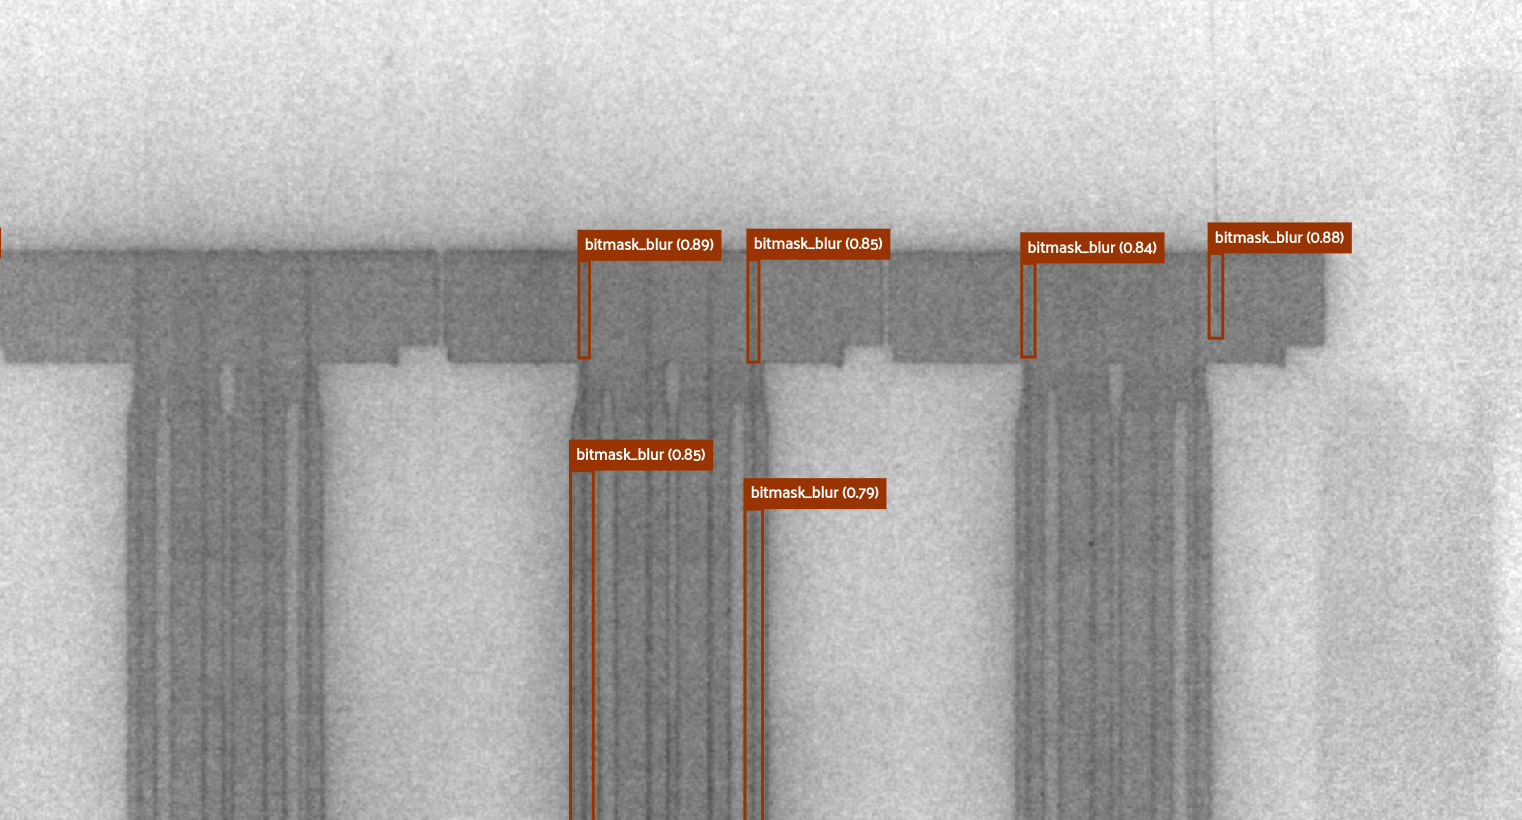
\includegraphics[width=\linewidth]{images/implementation/results/bm/bm_blur}
  \caption{Using a bitmask and it's blurred version}
\end{subfigure}

\begin{subfigure}{.6\textwidth}
  \centering
  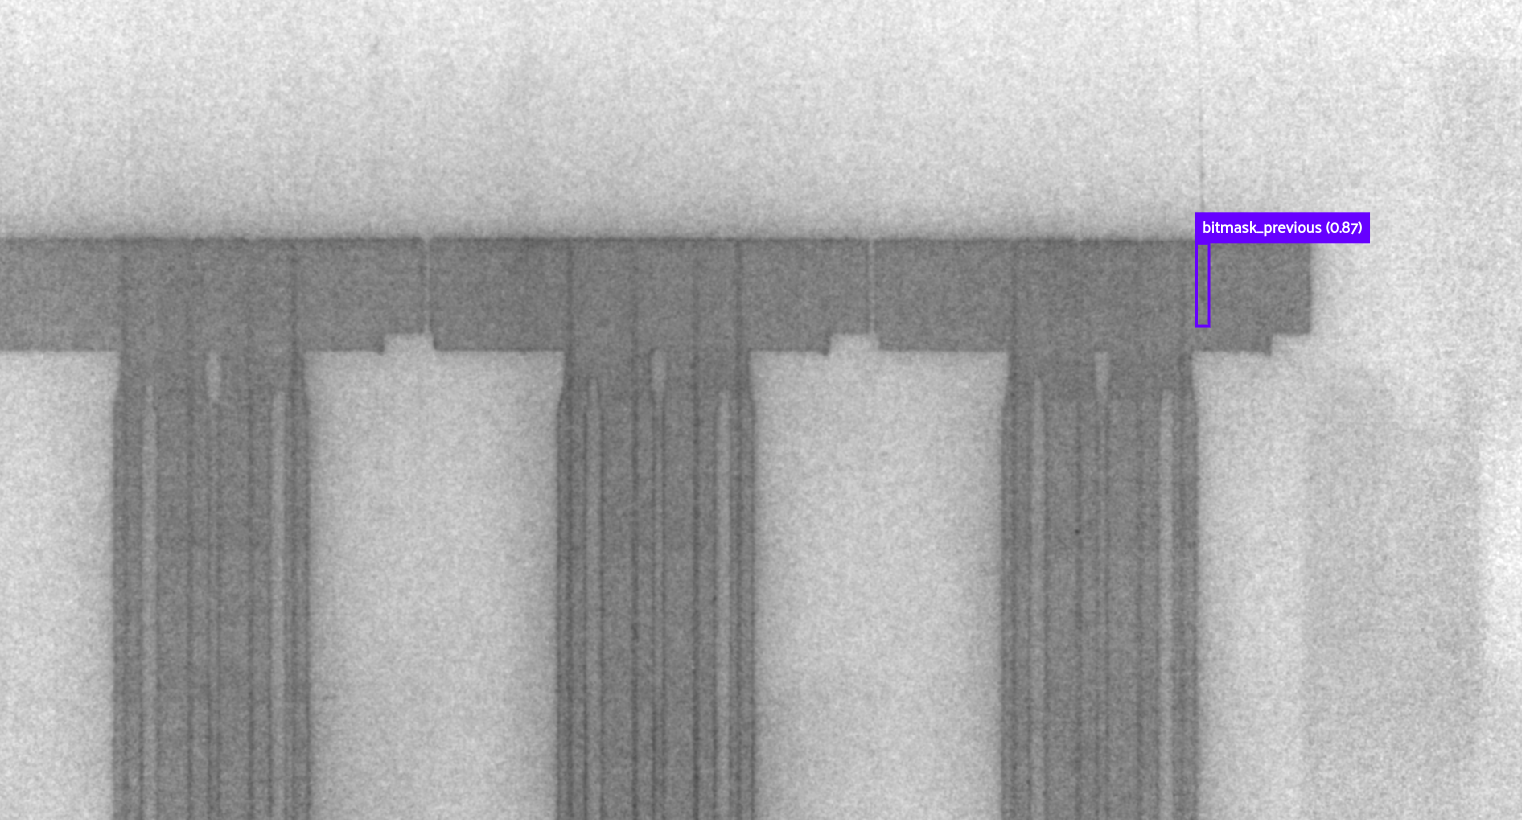
\includegraphics[width=\linewidth]{images/implementation/results/bm/bm_prev}
  \caption{Using current and previous bitmasks}
\end{subfigure}
\caption{The alternative methods tend to have many false positives. The best method that uses the current bitmask and previous bitmask and is therefore able to avoid the false detections. More examples in the appendix.}
\label{impl:bm_compare}
\end{figure}


The table bellow contains multiple metrics for individual bitmask integration methods. The recall rate is usually great, but the main difference is seen at the false positive count and implicitly precision metric.

\begin{table}[!h]
  \centering
    \begin{tabular}{ ||c|c|c|c|c|c||}
    \hline
    B channel & G channel & FP count & FN count & precision & recall\\ [0.5ex]
    \hline\hline
    bitmask & previous bitmask & 16 & 1 & 0.9 & 0.97 \\
    bitmask & logical OR of bitmasks & 37 & 3 & 0.67 & 0.93 \\
    bitmask & blurred bitmask & 25 & 2 & 0.85 & 0.95 \\
    bitmask & bitmask AND layer image & 13 & 2  & 0.75 & 0.95 \\
    \hline
    \end{tabular}
  \caption{Bitmask integration methods comparison}
  \label{wadfds}
\end{table}

Moreover, the recall rate barely changes for most methods across multiple confidence thresholds. This result is displayed in the table below.

\begin{table}[!h]
  \centering
    \begin{tabular}{ ||c|c|c|c|c|c||}
    \hline
    B channel & G channel & 0.2 & 0.4 & 0.6 & 0.8\\ [0.5ex]
    \hline\hline
    bitmask & previous bitmask & 0 & 1 & 1 & 1 \\
    bitmask & logical OR of bitmasks & 0 & 2 & 3 & 3 \\
    bitmask & blurred bitmask & 0 & 1 & 2 & 2 \\
    bitmask & bitmask AND layer image & 0 & 0 & 2 & 2 \\
    \hline
    \end{tabular}
  \caption{False negative count change across multiple confidence thresholds.}
  \label{wadfds23}
\end{table}

On the other hand, the false positive count decreases rapidly for each confidence threshold increase. See table \ref{impl:fp_count}.

\begin{table}[!h]
  \centering
    \begin{tabular}{ ||c|c|c|c|c|c||}
    \hline
    B channel & G channel & 0.2 & 0.4 & 0.6 & 0.8\\ [0.5ex]
    \hline\hline
    bitmask & previous bitmask & 138 & 77 & 35 & 18 \\
    bitmask & logical OR of bitmasks & 169 & 108 & 72 & 40 \\
    bitmask & blurred bitmask & 214 & 202 & 131 & 27 \\
    bitmask & bitmask AND layer image & 186 & 139 & 85 & 30 \\
    \hline
    \end{tabular}
  \caption{False positive count change across multiple confidence thresholds.}
  \label{impl:fp_count}
\end{table}

\textbf{Windowing}

In multiple head-to-head comparison the 2 strategies traded victories. One important remark is that the grid windowing strategy was actually very stable and the metrics barely fluctuated. This is because the actual windows never change. Meanwhile, the random windowing strategy fluctuates with a standard deviation of 0.1, which is far bigger than the 0.02 provided by the grid windowing. This is mostly, because the randomness can be sometimes very unlucky and for example split multiple scratches. For the next results the bitmask integration method is the one that contains both bitmasks.\\

\begin{table}
\centering
\begin{tabular}{ ||c|c|c|c|c||}
\hline
windowing method & average mAP@0.5 & min mAP & max mAP & std. deviation\\ [0.5ex]
\hline\hline
random windowing & 0.8 & 0.68 & 0.91 & 0.1 \\
grid windowing & 0.84  & 0.82 & 0.89 & 0.02 \\
double windowing & 0.81  & 0.78 & 0.83 & 0.02 \\
\hline
\end{tabular}
\caption{Overview of the stability of different windowing strategies/methods. The individual results are obtained by experiments with square windows of size 320, 640, 960 and 1280.}
\label{impl:win_strategy}
\end{table}

A more interesting result is the mAP@0.5:0.95 for different window sizes. The table below shows the results.


\begin{table}
\centering
\begin{tabular}{ ||c|c|c|c|c|c||}
\hline
window size & FP count & FN count & precision & recall & box loss\\ [0.5ex]
\hline\hline
320x320 & 28 & 0 & 0.85 & 1 & 0.07\\
640x640 & 19 & 2 & 0.89 & 0.95 & 0.05\\
960x960 & 11 & 3 & 0.93 & 0.9 & 0.02\\
1280x1280 & 9 & 3 & 0.96 & 0.9 & 0.02\\
\hline
\end{tabular}
\caption{Results of using different window sizes. The box loss is calculated during training and it's calculation is based on the IoU. This loss shows how good the bounding boxes of the detections are fitted. }
\label{impl:win_size}
\end{table}

The higher windows provide a better precision of a slightly worse recall. The problem of smaller windows is that they have a weaker bounding box fitting and the model tends to use multiple bounding boxes for the same detection. This is seen in figure \ref{impl:win_bb_compare}.

\begin{figure}[!h]
\centering
\begin{subfigure}{.5\textwidth}
  \centering
  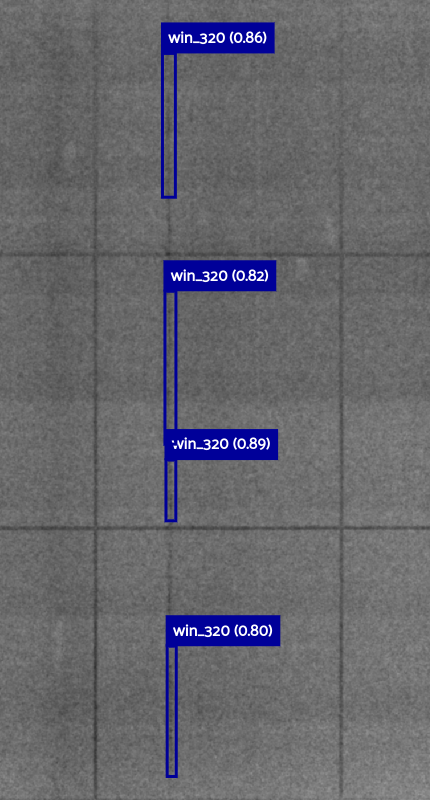
\includegraphics[width=\linewidth]{images/implementation/results/win/320}
  \caption{320x320 windows}
\end{subfigure}%
\begin{subfigure}{.5\textwidth}
  \centering
  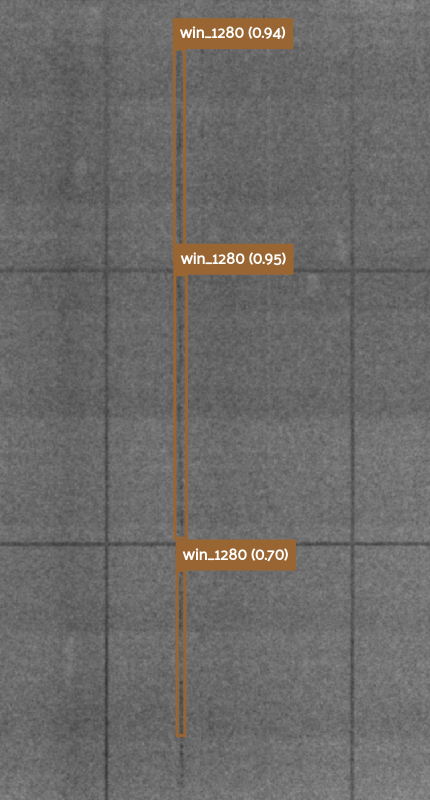
\includegraphics[width=\linewidth]{images/implementation/results/win/1280}
  \caption{1280x1280 windows}
\end{subfigure}
\caption{Larger windows tend to have less double detections and are able to better fit the bounding boxes.}
\label{impl:win_bb_compare}
\end{figure}


\textbf{Two Stage Training} \\
In section \ref{subsection:two_stage_training} two variations of the same approach have been presented. As a reminder, the difference is that one uses a on the second stage a single class and introduces the windows containing false positives in the dataset, while the other one marks the false positives as a second class in the second stage. The trade-off is that the two class approach was harder to track during training, while the one class approach did not had this kind of problems.
The results of the two stage training approach are summarized in the table below: \\
\begin{table}
  \centering
    \begin{tabular}{||c|c|c|c|c|c||}
    \hline
    Mode & FP count & FN count & FP count & precision & recall\\ [0.5ex]
    \hline\hline
    first stage & 0 & 0 & 0 & 0 \\
    first stage & 0 & 0 & 0 & 0 \\
    first stage & 0 & 0 & 0 & 0 \\
    \hline
    \end{tabular}
  \caption{asdf}
  \label{impl:two_stage_table}
\end{table}

WIP \\
Hier will ich die FPs, FNs, precision und recall zwischen den 2 two stage training methoden zeigen. \\

\textbf{Hyperparameter Optimization} \\
WIP \\
Muss eine gute strukturierung finden. \\

\textbf{Putting it all together (oder Final Result?)} \\
WIP \\
Hier will ich die beste Konfiguration zeigen \\
Folgendes wird hier sein:\\
  - confusion matrix \\
  - tabelle mit alle hyperparameters \\
  - tabelle mit FPs, FNs, precision, recall, mAP \\
  - workflow chart figure ref{impl:workflow}\\

\begin{figure}[!h]
  \centering
  \captionsetup{justification=centering,margin=2cm}
  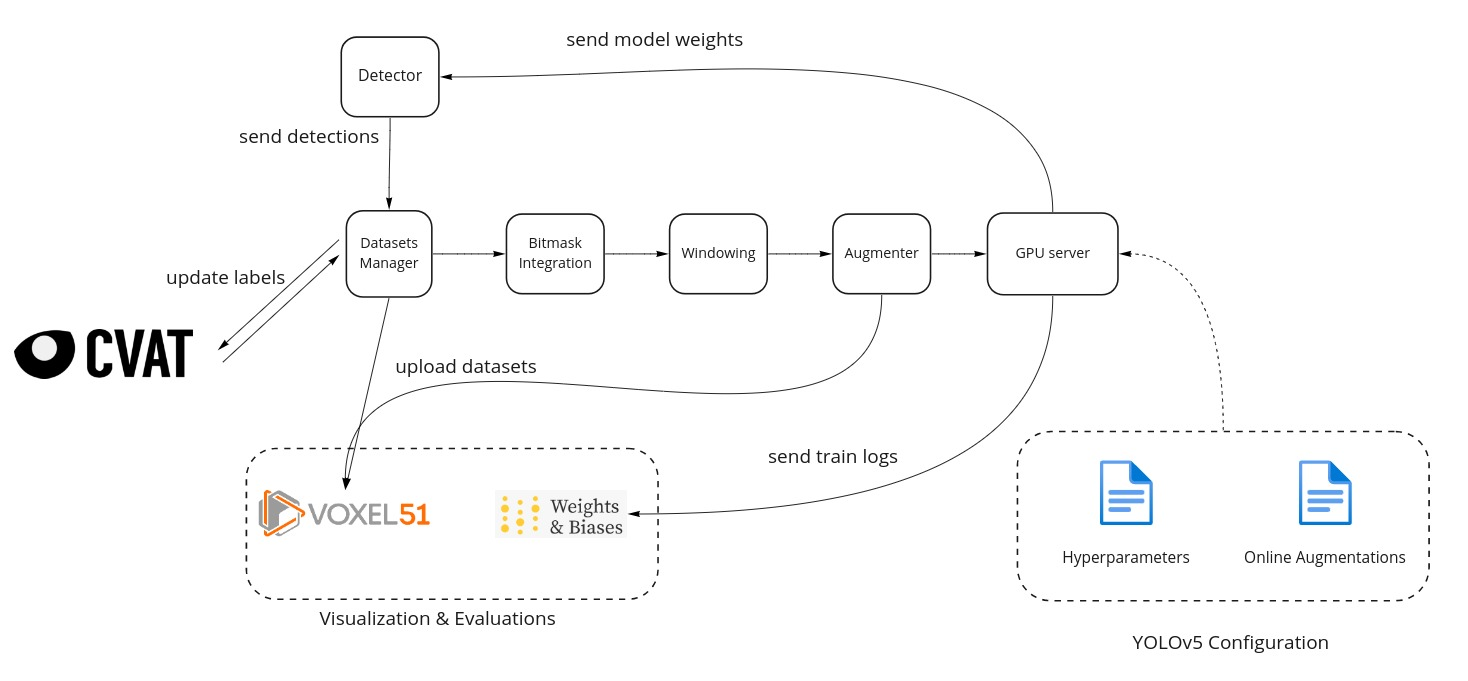
\includegraphics[width=\columnwidth]{images/implementation/results/workflow}
  \caption{Workflow}
  \label{impl:workflow}
\end{figure}


\subsection{Development Environment}
The scope of this section is to highlight some nice features of the used tools that were helpful during the development process. One important tool was FiftyOne \cite{fiftyone_git}, which can be used for dataset versioning and visualization. This tool supports advanced visualization filters and dataset format conversion. In the beginning, multiple YOLO versions were tested and each of them had a slightly different format and with FiftyOne the datasets could be quickly converted. The FifityOne filters could be use to see only a subset of the detections e.g. low confidence detections and it helped understand the consequences of different approaches.  \\
For annotation CVAT was great in combination with FiftyOne, because datasets in any format could be uploaded directly to CVAT server. After the annotation process is finished, the newly annotated datasets could be imported back into FiftyOne's database. \\
For logging Weights \& Biases is used, because YOLOv5 has integrated support for this platform. With Weights \& Biases it is easier to share training results and generate figure of training reports. A YOLOv5 specific logging feature is the \textit{Bounding Box Debugger}, which can be used to see how the model predicts on the validation set for every epoch that saves the weights. This feature is very helpful for the two stage training, when metrics and loss results lose meaning. \\
% TODO BB debugger fig here \\
A great alternative is CoreML, which is supported also by YOLOv5. The classic Tensorboard tool works too, but the limited features makes it difficult to work with a higher number of experiments. \\
